\documentclass[11pt, oneside]{book}

%%%%%%%%%%%%%%%%%%%%%%%%%%%%%%%%%%%%%%%%
%% Paquetes
\usepackage[spanish,es-ucroman,es-tabla]{babel}
\usepackage[T1]{fontenc}
\usepackage[utf8]{inputenc}
\usepackage{arev}
\usepackage{xcolor}
\usepackage{amsmath}
\usepackage{booktabs}
\usepackage{graphicx}
\usepackage[a4paper,left=3.5cm,right=2.0cm,top=1.2cm,
            headsep=3mm,headheight=2.3cm,includehead,
            footskip=15mm]{geometry}
\usepackage{float}
\usepackage{listings}
    \renewcommand{\lstlistingname}{Código}
\usepackage{setspace}
    \setstretch{1.15}
\usepackage{enumitem}
\usepackage[colorlinks,allcolors=.,breaklinks]{hyperref}
\usepackage{silence}
\WarningFilter{spanish}{Replacing `T1/fav/b/sc'}

%%%%%%%%%%%%%%%%%%%%%%%%%%%%%%%%%%%%%%%%
%% Colores
\color[HTML]{000078}
\definecolor{celeste}{HTML}{73EDFF}
\definecolor{gris}{HTML}{F0F0F0}


\makeatletter

%%%%%%%%%%%%%%%%%%%%%%%%%%%%%%%%%%%%%%%%
%% Encabezados y pies de página
\usepackage{fancyhdr}
    \fancyhf{}
    \renewcommand{\headrulewidth}{0pt}
    \fancyhead[L]{\hspace*{-2.5cm}
    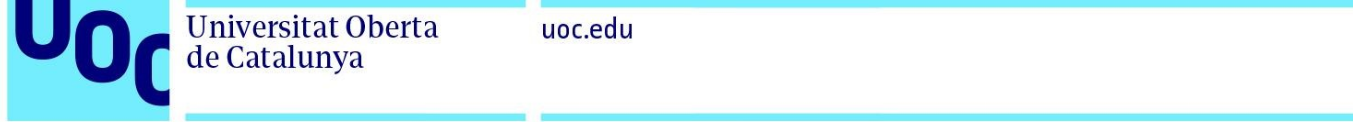
\includegraphics[width=18cm]{Figuras/encabezado.png}
    }
    \fancyfoot[R]{\footnotesize
    \begin{tabular}{@{}l@{\ \ }l@{\ \ }l@{}}
    \textcolor[HTML]{73EDFF}{\rule{6.7cm}{0.9mm}} &
    \textcolor[HTML]{73EDFF}{\rule{5.7cm}{0.9mm}} &
    \textcolor[HTML]{73EDFF}{\rule{2.7cm}{0.9mm}} \\
       \@programa  & \@fecha & \textbf{pág. \thepage}
    \end{tabular}
    }
\pagestyle{fancy}

\fancypagestyle{plain}{%
    \fancyhf{}
    \renewcommand{\headrulewidth}{0pt}
    \fancyhead[L]{\hspace*{-2.5cm}
    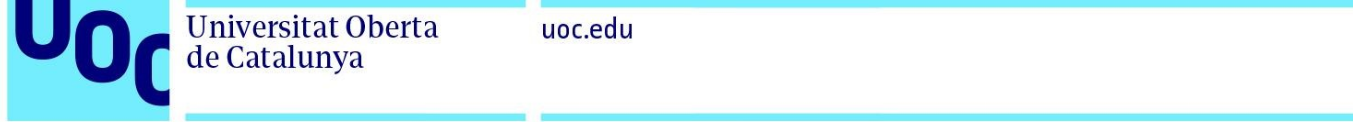
\includegraphics[width=18cm]{Figuras/encabezado.png}
    }
    \fancyfoot[R]{\footnotesize
    \begin{tabular}{@{}l@{\ \ }l@{\ \ }l@{}}
    \textcolor[HTML]{73EDFF}{\rule{6.7cm}{0.9mm}} &
    \textcolor[HTML]{73EDFF}{\rule{5.7cm}{0.9mm}} &
    \textcolor[HTML]{73EDFF}{\rule{2.7cm}{0.9mm}} \\
       \@programa  & \@fecha & \textbf{pág. \thepage}
    \end{tabular}
    }
}


%%%%%%%%%%%%%%%%%%%%%%%%%%%%%%%%%%%%%%%%
%% Datos
\newcommand{\@titulo}{}
\newcommand{\@tamtitulo}{}
\newcommand{\@subtitulo}{}
\newcommand{\@tamsubtitulo}{}
\newcommand{\@autor}{}
\newcommand{\@programa}{}
\newcommand{\@area}{}
\newcommand{\@tutor}{}
\newcommand{\@profesor}{}
\newcommand{\@idioma}{}
\newcommand{\@palabrasclave}{}
\newcommand{\@fecha}{\today}

\newcommand{\titulo}[2][45pt]{
    \renewcommand{\@tamtitulo}{#1}
    \renewcommand{\@titulo}{#2}}
\newcommand{\subtitulo}[2][35pt]{
    \renewcommand{\@subtitulo}{#1}
    \renewcommand{\@subtitulo}{#2}}
\newcommand{\autor}[1]{
    \renewcommand{\@autor}{#1}}
\newcommand{\programa}[1]{
    \renewcommand{\@programa}{#1}}
\newcommand{\area}[1]{
    \renewcommand{\@area}{#1}}
\newcommand{\tutor}[1]{
    \renewcommand{\@tutor}{#1}}
\newcommand{\profesor}[1]{
    \renewcommand{\@profesor}{#1}}
\newcommand{\fecha}[1]{
    \renewcommand{\@fecha}{#1}}
\newcommand{\idioma}[1]{
    \renewcommand{\@idioma}{#1}}
\newcommand{\palabrasclave}[1]{
    \renewcommand{\@palabrasclave}{#1}}

%%%%%%%%%%%%%%%%%%%%%%%%%%%%%%%%%%%%%%%%
%% Portada
\newcommand{\portada}{
    \newgeometry{margin=10mm}
    \thispagestyle{empty}
    \noindent
    \fcolorbox{celeste}{celeste}{
    \begin{minipage}[t][8.5cm][t]{18.5cm}
    \flushleft
    \hspace{0pt}\\
    {\fontsize{\@tamtitulo}{\@tamtitulo}\selectfont \textbf{\@titulo} \\}
    \vspace{\fill}
    \ifdefstring{\@subtitulo}{}{}%
    {\fontsize{\@tamsubtitulo}{\@tamsubtitulo}\selectfont \@subtitulo \\\vspace{5mm}}
    \end{minipage}
    }\\[5mm]
    
\includegraphics[width=6.5cm]{Figuras/portada.png}
    \hspace{4mm}
    \fcolorbox{gris}{gris}{
    \begin{minipage}[b][17cm][t]{11.4cm}
    \flushleft
    \hspace{0pt}\\
    \Huge
    \textbf{\@autor}\\\vspace{\fill}
    \@programa\\\vspace{\fill}
    \textbf{Área:} \@area\\\vspace{\fill}
    \textbf{Tutor de TF:}\\
    \@tutor\\\vspace{\fill}
    \textbf{Profesor responsable de la asignatura:}\\
    \@profesor\\\vspace{\fill}
    \@fecha\\\vspace{\fill}
    \end{minipage}
    }
    
    \clearpage
    \restoregeometry

    \vspace*{\fill}
    \noindent
    \begin{minipage}{12cm}
    \flushleft
    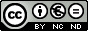
\includegraphics[width= 2.5cm]{Figuras/cc.png}\\
    Esta obra está sujeta a una licencia de Reconocimiento- NoComercial-SinObraDerivada \href{https://creativecommons.org/licenses/by-nc-nd/3.0/es/}{3.0 España de Creative Commons}
    \end{minipage}
    \vspace{2cm}

    \newpage

    \chapter*{Ficha del Trabajo Final}
\begin{center}
\begin{table}[ht]
	\centering{}
	\renewcommand{\arraystretch}{2}
	\begin{tabular}{|R{4.5cm} | L{10cm}|}
		\hline
		\textbf{Título del trabajo:} &\cellcolor{gris}\@titulo\\
		\hline
        \textbf{Nombre del autor:} &\cellcolor{gris}\@autor\\
		\hline
        \textbf{Nombre del Tutor de TF:} &\cellcolor{gris}\@tutor\\
		\hline
        \textbf{Fecha de entrega:} &\cellcolor{gris}\@fecha\\
		\hline
        \textbf{Titulación o programa:} &\cellcolor{gris}\@programa\\
		\hline
        \textbf{Área del Trabajo Final:} &\cellcolor{gris}\@area\\
		\hline
        \textbf{Idioma del trabajo:} &\cellcolor{gris}\@idioma\\
		\hline
        \textbf{Palabras clave:} &\cellcolor{gris}\@palabrasclave\\
		\hline
	\end{tabular}
\end{table}
\end{center}
}

%%%%%%%%%%%%%%%%%%%%%%%%%%%%%%%%%%%%%%%%
%% Bibliografía
% \usepackage[babel]{csquotes}
% \usepackage[style=apa,backend=biber]{biblatex}
%     \DeclareLanguageMapping{spanish}{spanish-apa}
    
%     \DefineBibliographyStrings{spanish}{%
%       andothers = {et al\adddot},
%     }
    
%     \DefineBibliographyExtras{spanish}
%         {\setcounter{smartand}{1}% or some other value
%          \let\lbx@finalnamedelim=\lbx@es@smartand
%          \let\lbx@finallistdelim=\lbx@es@smartand}
    
%     \setlength{\bibhang}{\parindent}  

%%%%%%%%%%%%%%%%%%%%%%%%%%%%%%%%%%%%%%%%
%% Leyendas
\usepackage[font={small},labelfont={bf,small},
  justification=centerlast,tablename=Tabla]{caption}

%%%%%%%%%%%%%%%%%%%%%%%%%%%%%%%%%%%%%%%%
%% Código
\definecolor{codegreen}{rgb}{0,0.6,0}
\definecolor{codegray}{rgb}{0.5,0.5,0.5}
\definecolor{codepurple}{rgb}{0.58,0,0.82}

\lstdefinestyle{mystyle}{
    backgroundcolor=\color{celeste!20},   
    commentstyle=\color{codegreen},
    keywordstyle=\color{magenta},
    numberstyle=\tiny\color{codegray},
    stringstyle=\color{codepurple},
    basicstyle=\ttfamily\footnotesize,
    breakatwhitespace=false,         
    breaklines=true,                 
    captionpos=b,                    
    keepspaces=true,                 
    numbers=left,                    
    numbersep=5pt,                  
    showspaces=false,                
    showstringspaces=false,
    showtabs=false,                  
    tabsize=2,
    linewidth=0.98\linewidth,
    xleftmargin=0.5cm
}

\lstset{style=mystyle}

%%%%%%%%%%%%%%%%%%%%%%%%%%%%%%%%%%%%%%%%
%% Tablas
\usepackage{array, multirow}
\newcolumntype{C}[1]{>{\hspace{0pt}\centering\arraybackslash}m{#1}}
\newcolumntype{L}[1]{>{\hspace{0pt}\arraybackslash}m{#1}}
\newcolumntype{R}[1]{>{\hspace{0pt}\raggedleft\arraybackslash}m{#1}}
\usepackage{colortbl}
\usepackage{longtable}
\setlength{\LTpost}{-25pt}

\colorlet{tableheadcolor}{celeste!50} % Table header colour = 25% gray
\newcommand{\topline}{\arrayrulecolor{black}\specialrule{\heavyrulewidth}{\abovetopsep}{0pt}%
            \arrayrulecolor{tableheadcolor}\specialrule{\belowrulesep}{0pt}{0pt}%
            \arrayrulecolor{black}}
\newcommand{\midline}{\arrayrulecolor{tableheadcolor}\specialrule{\aboverulesep}{0pt}{0pt}%
            \arrayrulecolor{black}\specialrule{\lightrulewidth}{0pt}{0pt}%
            \arrayrulecolor{white}\specialrule{\belowrulesep}{0pt}{0pt}%
            \arrayrulecolor{black}}


\makeatother
\usepackage{amsthm}
\usepackage{algorithm}
\usepackage{algorithmic}
\usepackage{tocloft}
\setlength{\cftfignumwidth}{2.55em}

\titulo[38.5pt]{Reconocimiento automático de imágenes para reconstrucción de redes planta-polinizador}
% \subtitulo{Subtítulo (si lo hay)}
\autor{Andrés Merino Toapanta}
\programa{Máster Universitario en Ciencias de Datos}
\area{Machine Learning}
\tutor{Albert Solé-Ribalta, Pau Enric Serra, Javier Borge Holthoefer}
\profesor{Albert Solé-Ribalta}
\idioma{Castellano}
\palabrasclave{Reconocimiento de imágenes, red planta-polinizador, red neuronal convolucional}
\fecha{Enero 2024}

% \addbibresource{referencias.bib}

\begin{document}


% portada
\frontmatter
\portada
% abstract
%%%%%%%%%%%%%%%%%%%
%%% DEDICATORIA %%%
%%%%%%%%%%%%%%%%%%%
\chapter*{}

\begin{raggedleft}
    \itshape La Ciencia de Datos\\ es un invento de los matemáticos\\ para vender más Matemática.\\
\end{raggedleft}

%%%%%%%%%%%%%%%%%%%
%%% Agradecimientos %%%
%%%%%%%%%%%%%%%%%%%
\chapter*{Agradecimientos}

A mi familia, por sus enseñanzas y los valores que me supieron inculcar. Por las alegrías y problemas que me han llevado a donde ahora estoy. A mis padres, mis hermanas y mi cuñado por el amor y el cariño que han compartido conmigo.

\vspace{\baselineskip}

A mis tutores: Albert Solé-Ribalta, Pau Enric Serra, Javier Borge
Holthoefer, por proponer el problema de este trabajo, por su apoyo y guía durante el desarrollo de este trabajo.

\vspace{\baselineskip}

A Janeth y Mario, quienes me han acompañado en este camino, me motivaron a iniciarlo y me han brindado su apoyo y cariño.

\vspace{\baselineskip}

A mis alumnos, en especial a Melani, Sofía, Martín y Pancho, quienes me ayudan a seguir descubriendo los hermoso del camino de aprender y enseñar. 

\vspace{\baselineskip}

A todos mis amigos (Priss, Eve, Cristian, David, Pau, Mishu,\dots), que cerca o lejos, siempre están ahí para compartir un momento, una charla, un café, una cerveza, una sonrisa, un abrazo, un consejo, una vida.

%%%%%%%%%%%%%%%%
%%% RESUMEN  %%%
%%%%%%%%%%%%%%%%
\chapter*{Abstract}
\addcontentsline{toc}{chapter}{Abstract}

\onehalfspacing

The present work focuses on the construction and training of a convolutional neural network (CNN) with the main objective of detecting pollinators in flower images, which will serve as a basis for the reconstruction of plant-pollinator interaction networks. Specific objectives include the collection and labeling of around 5,000 images of pollinators in two study habitats in Cabrera, Balearic Islands; evaluation of two convolutional neural network architectures (YOLOv5 and EfficientNET) for accurate pollinator detection (in functional groups), training of the selected network, reconstruction of a pollination network from the detections, and performance evaluation using standard network metrics. With the results of this work, we seek to automate the collection and classification of interactions, directly delivering the plant-pollinator interaction network, which offers valuable information both for new research and for decision-making regarding agriculture and conservation.

\vspace{1.5cm}

\paragraph{Keywords:} Image recognition, plant-pollinator network, convolutional neural network.

%%%%%%%%%%%%%%%%
%%% RESUMEN  %%%
%%%%%%%%%%%%%%%%
\chapter*{Resumen}
\addcontentsline{toc}{chapter}{Resumen}

\onehalfspacing

El presente trabajo se centra en la construcción y entrenamiento de una red neuronal convolucional (CNN) con el objetivo principal de detectar polinizadores en imágenes de flores, lo que servirá como base para la reconstrucción de redes de interacción planta-polinizador. Los objetivos específicos incluyen la recopilación y etiquetado de alrededor de 5000 imágenes de polinizadores en dos hábitats de estudio en Cabrera, Islas Baleares; la evaluación de dos arquitecturas de redes neuronales convolucionales (YOLOv5 y EfficientNET) para la detección precisa de polinizadores (en grupos funcionales), el entrenamiento de la red seleccionada, la reconstrucción de una red de polinización a partir de las detecciones y la evaluación del desempeño utilizando métricas estándar sobre la red. Con los resultados de este trabajo, se busca poder automatizar la recolección y clasificación interacciones, entregando directamente la red de interacción planta-polinizador, que ofrezca información valiosa tanto para nuevas investigaciones como para la toma de decisiones en lo referente a agricultura y conservación.



\vspace{1.5cm}

\paragraph{Palabras clave:} Reconocimiento de imágenes, red planta-polinizador, red neuronal convolucional. 
\newpage

% indice
\addcontentsline{toc}{chapter}{Índice}
\tableofcontents
% listado de figuras
\newpage
\addcontentsline{toc}{chapter}{Listado de Figuras}
% cambio el nombre de la lista de figuras
\renewcommand{\listfigurename}{Listado de Figuras}
\listoffigures
% listado de tablas
% cambio el nombre de la lista de tablas
\renewcommand{\listtablename}{Listado de Tablas}
\newpage
\addcontentsline{toc}{chapter}{Listado de Tablas}
\listoftables



\mainmatter
% capitulos del documento
\chapter{Introducción}
\label{chapter:introduccion}


%%% SECTION
\section{Contexto y justificación del trabajo}

La polinización es un proceso crucial para la reproducción de muchas especies vegetales, incluyendo cultivos agrícolas de importancia económica, de hecho, tres cuartos (75\%) de los 111 cultivos agrícolas más importantes en todo el mundo dependen, en mayor o menor medida, de la polinización realizada por animales \cite{klein-2006}. 

Los polinizadores, como las abejas, mariposas, pájaros y murciélagos, desempeñan un papel esencial en la transferencia de polen de una flor a otra, permitiendo la fertilización y la producción de frutas y semillas. De todos estos animales, los insectos son los polinizadores más importantes, ya que son responsables de la polinización de más del 67\% de las especies de plantas con flores en todo el mundo \cite{innovatione-agrofood-design-2021}.

Sin embargo, en las últimas décadas, ha habido una disminución preocupante en la población de polinizadores debido a factores como la pérdida de hábitat, el uso de pesticidas y el cambio climático \cite{unam-2019}. Esto plantea una amenaza significativa para la seguridad alimentaria y la biodiversidad global.

Para abordar esta problemática, es crucial comprender y monitorear la actividad de los polinizadores en diferentes entornos. La observación directa y el seguimiento manual de los polinizadores pueden ser costosos y laboriosos. Aquí es donde entra en juego la tecnología de visión por computadora y las redes neuronales convolucionales.

La detección de polinizadores a partir de imágenes utilizando redes neuronales convolucionales ofrece numerosos beneficios como por ejemplo:

\begin{itemize}
    \item 
    \textbf{Eficiencia y Escalabilidad:} Las redes neuronales convolucionales permiten procesar grandes conjuntos de datos de imágenes de manera eficiente y automatizada. Esto significa que es posible recolectar y analizar todas las interacciones en una cantidad significativa de datos en un corto período de tiempo, lo que facilita la monitorización a largo plazo.
    
    \item 
    \textbf{Precisión:} Las CNN son conocidas por su capacidad para detectar patrones y características en imágenes con alta precisión. Esto garantiza que las detecciones de polinizadores sean confiables y consistentes.
    
    \item 
    \textbf{Aplicabilidad:} Este enfoque puede ser aplicado en una variedad de entornos, desde campos agrícolas hasta áreas naturales, lo que lo hace relevante tanto para la investigación científica como para la toma de decisiones en agricultura y conservación.
\end{itemize}

El objetivo de este trabajo es utilizar redes neuronales convolucionales para construir un modelo que habilite la detección de polinizadores y los clasifique en grupos funcionales, con lo que se pueda reconstruir una red de polinización. De esta manera, se podrá monitorear la actividad de los polinizadores en diferentes entornos y se podrá identificar tendencias en las poblaciones de polinizadores. Esto brindará información valiosa para las instituciones de investigación como para los diferentes departamentos gubernamentales y no gubernamentales en la toma de decisiones para la agricultura y la conservación.



\section{Motivación}

Mi trayectoria como docente e investigador en la Facultad de Ciencias Exactas y Naturales de la Pontificia Universidad Católica del Ecuador se ha enriquecido significativamente gracias a la colaboración interdisciplinaria con colegas de la Escuela de Biología. Estas sinergias han abierto oportunidades únicas para integrar mi especialización en matemáticas y ciencia de datos con el estudio y la preservación de la biodiversidad ecuatoriana, un campo de vital importancia en un país que se distingue por ser el sexto más megadiverso del mundo.

La interacción con estas diversas disciplinas me ha permitido acompañar a estudiantes tanto de Biología como de Ciencia de Datos en salidas de campo, donde la teoría se encuentra con la práctica. Estas experiencias en el terreno han sido fundamentales para comprender la complejidad y la riqueza de las especies de nuestro país, muchas de las cuales aún están por descubrir. Esta inmersión directa en el estudio de la biodiversidad ha fortalecido mi convicción de que la conservación efectiva requiere de enfoques innovadores y técnicas avanzadas, como el reconocimiento automático de imágenes, para enfrentar los desafíos emergentes como la deforestación, la caza furtiva, la contaminación y el cambio climático.

A través de este trabajo, se busca contribuir con un enfoque que permita la reconstrucción de redes de polinización de manera más eficiente y no invasiva. La meta es proporcionar herramientas que mejoren nuestra capacidad de monitoreo y protección de las especies, particularmente en extensas áreas donde la aparición de nuevas especies requiere una rápida inclusión en los planes de conservación. Este proyecto representa la confluencia de mi experiencia en el aula y en el campo, mi colaboración con expertos en Biología y mi formación en Ciencia de Datos, todo dirigido hacia un objetivo común: proteger y entender mejor el tesoro natural que Ecuador posee.

\section{Objetivos}

\subsection{Objetivo principal}

Construir y entrenar una red neuronal convolucional para la detección de polinizadores en imágenes de flores, que sirva de manera universal para la reconstrucción de redes de polinización. 

\subsection{Objetivos específicos}

\begin{itemize}
    \item Depurar un conjunto de datos de imágenes de polinizadores.
    \item Seleccionar un modelo de red neuronal convolucional para la detección de polinizadores en imágenes.
    \item Entrenar la red neuronal convolucional sobre el conjunto de datos de imágenes de polinizadores construida.
    \item Reconstruir una red de polinización a partir de las detecciones de la red neuronal convolucional.
    \item Evaluar los resultados analizando las métricas de la red de polinizadores reconstruida.
\end{itemize}

\section{Metodología}

Como es usual en los proyectos de Ciencia de Datos, el proyecto se divide en las siguientes etapas: recopilación y preparación de datos, creación de modelo a aplicarse sobre los datos y evaluación contextualizada de los resultados obtenidos.

En lo que respecta a la recopilación y preparación de datos, se utilizará un conjunto de alrededor de cinco mil imágenes (5000) registradas en dos hábitats y cuatro lugares de estudio en Cabrera (Islas Baleares, ver Figura \ref{fig:ubicacion}). Los polinizadores están identificados por expertos y etiquetados utilizando las siguientes categorías: «Bee», «Diptera», «Coleoptera», «Hoverfly», «Lepidoptera», «Wasp» y «Others». 

\begin{figure}[H]
    \centering
    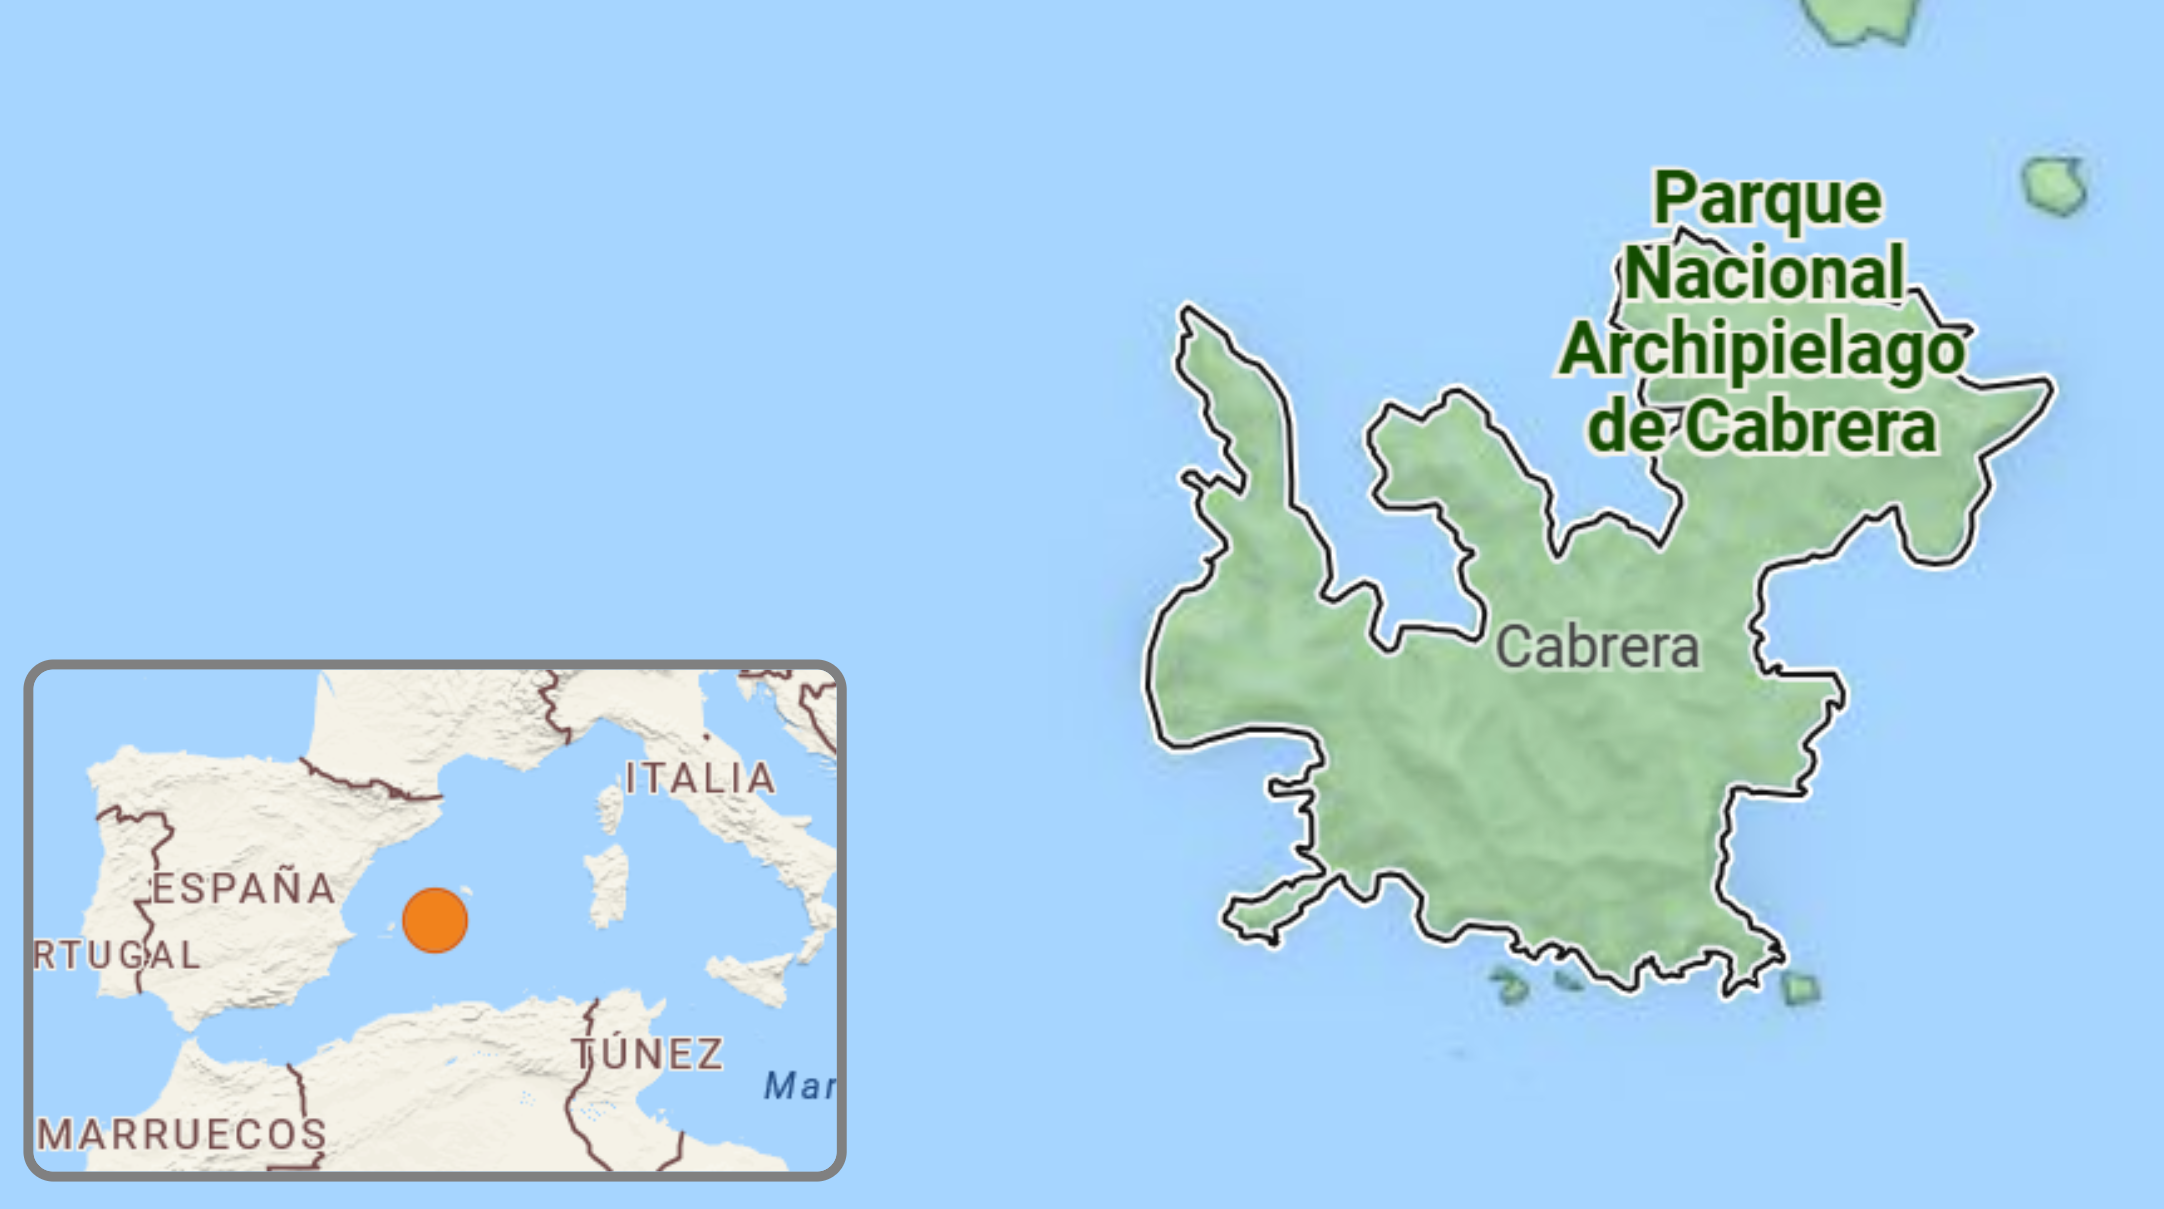
\includegraphics[width=0.9\textwidth]{Figuras/ubicacion.png}
    \caption[Ubicación de Cabrera.]{Ubicación de Cabrera. Tomado de Bing \cite{bing_maps}}
    \label{fig:ubicacion}
\end{figure}

Para realizar la identificación de las plantas que se hallan en el fondo de las imágenes, se utilizará la herramienta \textit{My PlantNet API} \cite{PlantNet}. Se planteará la identificación a nivel de Familia, para, de esta manera, obtener los grupos de plantas que cada insecto poliniza.

Esta será la etapa de partida para la construcción del conjunto de datos de imágenes de polinizadores que será utilizado para el entrenamiento y evaluación de las etapas posteriores. Finalmente, de darse el caso, se utilizarán técnicas tradicionales de aumento de imágenes para incrementar el tamaño del conjunto de datos; entre estas, se encuentran la rotación, el recorte, el volteo, el cambio de color, etc.


Por el lado del diseño de una red neuronal convolucional para la detección de polinizadores en imágenes, se analizarán dos alternativas: la arquitectura de red neuronal convolucional \textit{YOLOv5}  que ha demostrado dar buenos resultados en la detección de objetos en imágenes, en especial, de insectos \cite{ahmad-2022,qi-2023}; y la arquitectura de red neuronal convolucional \textit{EfficientNET} que ha obtenido resultados de precisión altos cuando se trata de pocas clases \cite{monis-2022}.

En lo relacionado con la evaluación contextualizada de los resultados obtenidos, en primera instancia, se utilizarán las métricas de precisión, sensibilidad y especificidad para evaluar el desempeño de la red neuronal convolucional. Además, a partir de los resultados, se reconstruirá una red de polinización bajo la metodología descrita en \cite{young-2021} y se analizarán las métricas de la misma.

Finalmente, en lo que respecta a la documentación del proyecto, se utilizará el lenguaje de programación Python y el entorno de desarrollo Jupyter Notebook. En específico, se utilizará la librería \textit{Tensorflow} y \textit{Pytorch} para la construcción de la red neuronal convolucional y la librería \textit{NetworkX} para el análisis y visualización de la red de polinización. El código fuente del proyecto se encontrará disponible en el repositorio de GitHub (ver Anexo \ref{anexo:github}). Adicionalmente, los pesos de los modelos entrenados se encontrarán disponibles en el repositorio particular de OneDrive del autor (ver Anexo \ref{anexo:pesos}).

\section{Planificación}

En la Figura \ref{fig:plan} se muestra el diagrama Gantt de la propuesta de planificación de las diferentes actividades del proyecto.

Las actividades del proyecto se agrupan en cuatro etapas: Definición y planificación del trabajo, Elaboración del estado del arte, Diseño e implementación del trabajo, Redacción de la memoria. Adicionalmente, se incluye una etapa de Defensa del trabajo.

Para la primera etapa, se estima una duración de 2 semanas. En esta etapa se realizará la definición de la propuesta, los objetivos y la metodología. Para la segunda etapa, se estima una duración de 3 semanas. En esta etapa se realizará la recolección de información y la redacción del estado del arte. Para la tercera etapa, se estima una duración de 8 semanas. En esta etapa se realizará la construcción del conjunto de datos, el diseño de la red neuronal, el entrenamiento de la red neuronal y la reconstrucción de la red de polinización; se finaliza con la evaluación de los resultados. Para la cuarta etapa, se estima una duración de 4 semanas. En esta etapa se realizará la redacción de la memoria. Finalmente, para la quinta etapa, se estima una duración de 1 semana. En esta etapa se realizará la defensa del trabajo.

De manera específica, en la Figura \ref{fig:plan} se aprecian la distribución de las actividades en el tiempo. Los rombos representas las fechas de entrega de avances del proyecto.

\begin{figure}[H]
    \centering
    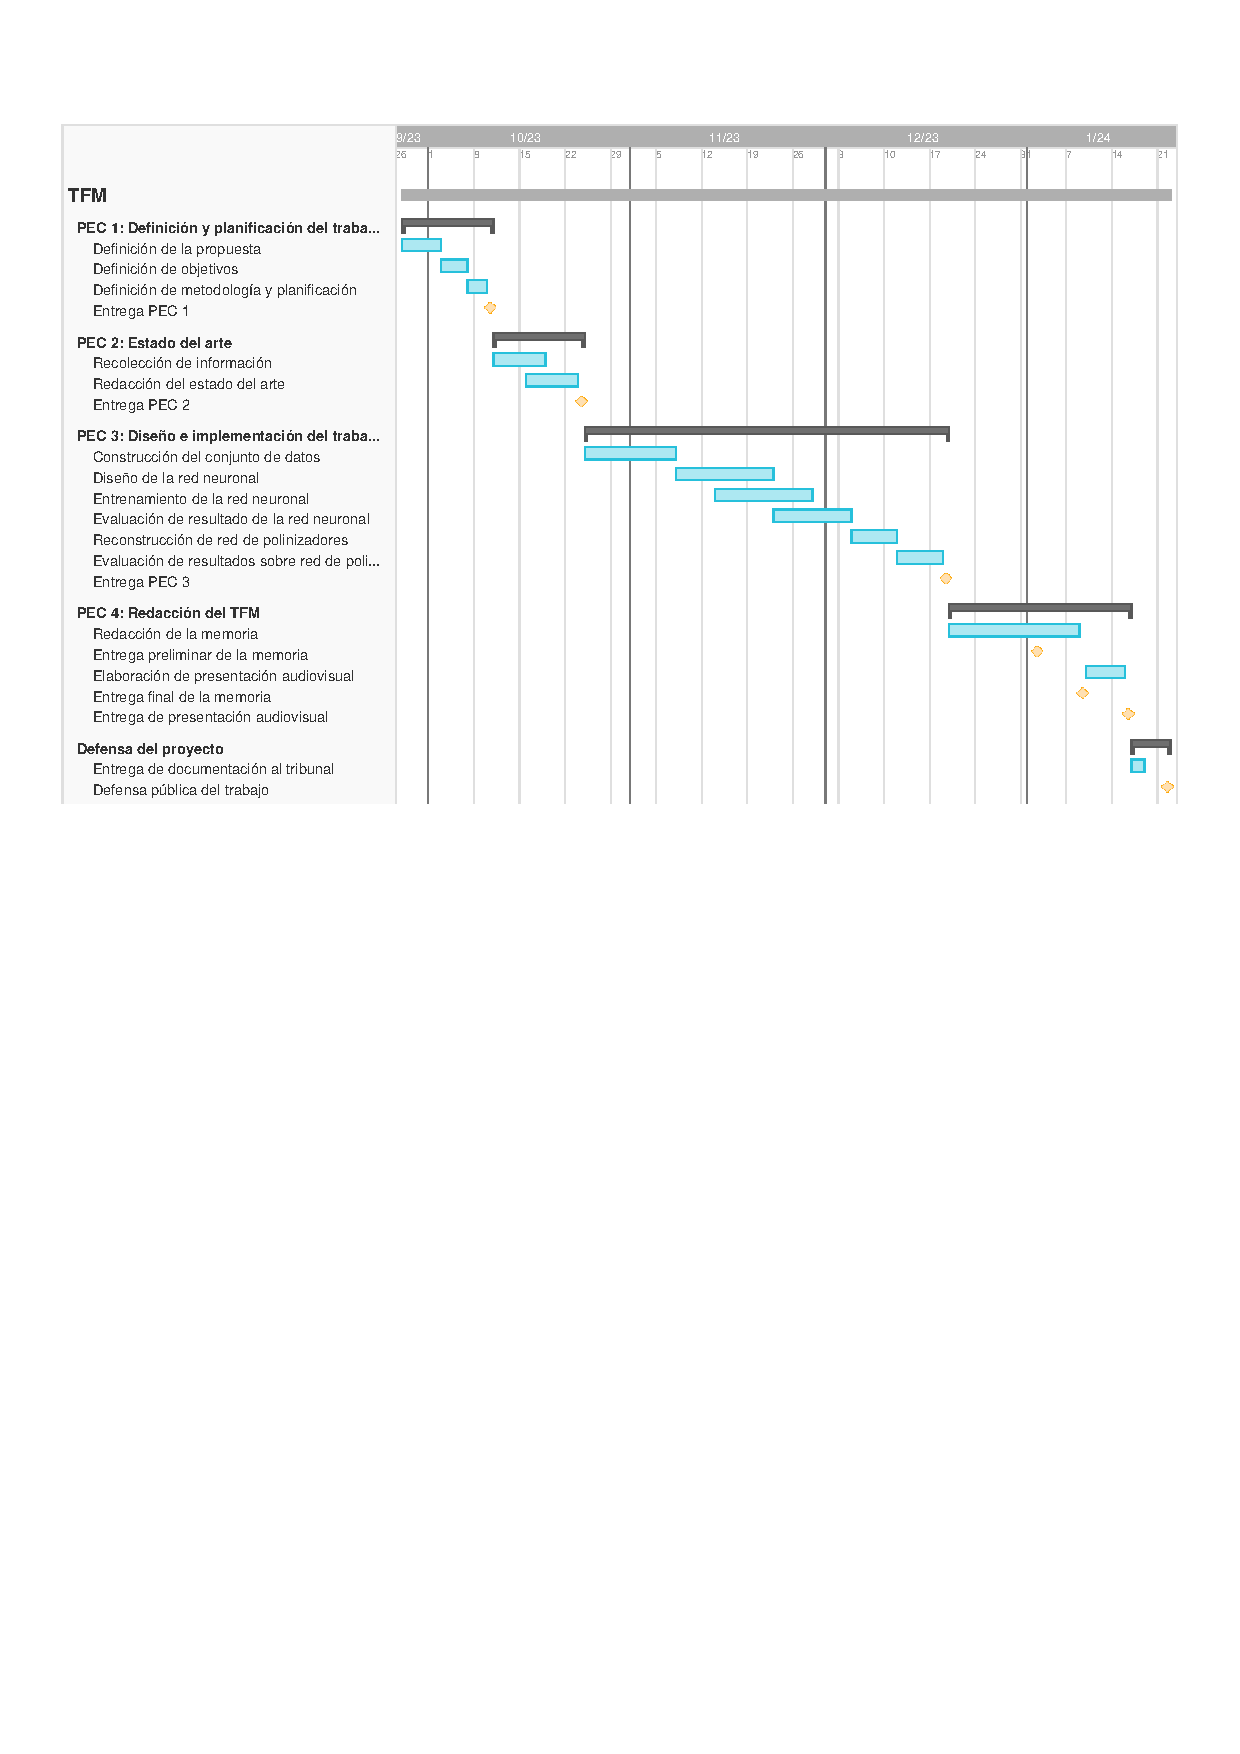
\includegraphics[width=1.44\textwidth,angle=90]{Figuras/PlanTFM.pdf}
    \caption{Diagrama Gantt de la planificación del proyecto.}
    \label{fig:plan}
\end{figure}


\section{Impacto en sostenibilidad, ético-social y de diversidad}

\paragraph{Sostenibilidad:} Este proyecto contribuye al ODS 15 (Vida de Ecosistemas Terrestres), ya que promueve la sostenibilidad de los ecosistemas terrestres. Al facilitar la monitorización y el estudio de los polinizadores, contribuye a la conservación de la biodiversidad y al mantenimiento de ecosistemas saludables, esenciales para la seguridad alimentaria y el equilibrio natural. Además, al emplear tecnologías de visión por computadora, reduce la necesidad de métodos de monitoreo invasivos y laboriosos, alineándose con prácticas sostenibles y de bajo impacto ambiental.

\paragraph{Comportamiento Ético y Responsabilidad Social:} Al mejorar la gestión de ecosistemas de polinizadores, este trabajo apoya indirectamente el ODS 2 (Hambre cero). Una identificación precisa de los polinizadores puede impulsar estrategias para optimizar prácticas agrícolas, aumentando la eficiencia de la polinización y mejorando los rendimientos de cultivos. Esto no solo fortalece la seguridad alimentaria, sino que también apoya prácticas agrícolas más éticas y sostenibles, contribuyendo al bienestar de las comunidades dependientes de la agricultura.

\paragraph{Diversidad, Género y Derechos Humanos:} Este proyecto contribuye al ODS 10 (Reducción de las desigualdades). La implementación de tecnologías de detección automática de polinizadores permite a países con recursos limitados acceder a información vital para la conservación de sus ecosistemas, equiparando su capacidad de cuidado y estudio de la biodiversidad con la de países de mayores recursos. Esto promueve una distribución más equitativa del conocimiento y las herramientas necesarias para la protección ambiental global.
\chapter{Estado del arte}
\label{chapter:arte}

En este capítulo se presentan los conceptos básicos de las redes neuronales convolucionales, así como los trabajos más relevantes en el campo de la detección de polinizadores a partir de imágenes utilizando este tipo de redes. Luego de esto, se expone lo referente al preprocesamiento de las imágenes. Posteriormente, se resume una metodología para realizar la reconstrucción de redes de polinización a partir de datos observacionales. Estas son las técnicas fundamentales que se van a usar en lo largo del proyecto.

\section{Reconocimiento de imágenes}

Se entiende por «reconocimiento de imágenes» a la tarea de identificar y localizar objetos en una imagen. Esta tarea se puede dividir en dos sub-tareas: clasificación y detección. La clasificación consiste en identificar el objeto en la imagen, mientras que la detección consiste en identificar su ubicación en la imagen (\textit{bounding box}). Para el caso de la clasificación, se tiene como entrada una imagen y se obtiene como salida una etiqueta que identifica el objeto en la imagen. Estas etiquetas pertenecen a un conjunto finito de categorías preestablecidas.

\section{Origen de las redes neuronales convolucionales}

Las redes neuronales convolucionales (CNN por sus siglas en ingles \textit{Convolutional Neural Network}) son un tipo de red neuronal artificial que se utiliza principalmente para el procesamiento de imágenes. Las CNN se inspiran en la corteza visual de los animales, específicamente en el sistema visual primario de los gatos, descrito por Hubel y Wiesel en 1962 \cite{hubel-1962}. En este sistema, las neuronas individuales responden a estímulos en regiones restringidas del campo visual conocidas como campos receptivos. Estas neuronas se organizan en capas, donde cada capa se compone de un conjunto de neuronas que responden a un campo receptivo específico. Las neuronas de la primera capa responden a estímulos simples, como líneas y bordes, mientras que las neuronas de capas posteriores responden a estímulos más complejos, como formas y objetos. Las neuronas de capas posteriores se activan cuando se activan las neuronas de capas anteriores, lo que permite la detección de características cada vez más complejas. Este proceso se conoce como extracción de características.

El inicio de las CNN se remonta a 1982, cuando Fukushima propuso la arquitectura Neocognitron \cite{fukushima-1982}, en la cual se presentaban células simples y complejas que sería el análogo a lo que actualmente se conoce como las capas de una CNN. No fue hasta 1989 cuando LeCun et al. \cite{lecun-1989} propusieron la arquitectura LeNet-5, que se considera la primera CNN moderna. Desde entonces, las CNN han sido ampliamente utilizadas en el campo del procesamiento de imágenes y en el reconocimiento de objetos.

El inicio de las CNN se remonta a 1982, cuando Fukushima propuso la arquitectura Neocognitron \cite{fukushima-1982}, sentando las bases para lo que más tarde serían las capas de una CNN. La evolución continuó en 1989 con LeCun et al. \cite{lecun-1989} y la introducción de la arquitectura LeNet-5, considerada la primera CNN moderna. Sin embargo, el verdadero salto hacia el Aprendizaje Profundo (\textit{Deep Learning}) se produjo en la última década, impulsado por varios factores clave.

El desarrollo de hardware más potente, especialmente GPUs, permitió el entrenamiento de redes neuronales más profundas y complejas \cite{alzubaidi-2021}. Paralelamente, avances en algoritmos y técnicas de entrenamiento, como la función de activación ReLU y la regularización mediante Dropout, optimizaron el proceso de aprendizaje para redes más profundas \cite{GU2018354}. La aparición de arquitecturas revolucionarias, como AlexNet en 2012 , demostró mejoras significativas en tareas de procesamiento de imágenes y reconocimiento de objetos \cite{russakovsky-2015}.


\subsection{Arquitectura y conjuntos de entrenamiento}

En la actualidad, existen varias arquitecturas que han dado buenos resultados en el campo del reconocimiento de objetos en imágenes. Algunas de estas son: AlexNet \cite{russakovsky-2015}, VGGNet \cite{simonyan2014very}, GoogLeNet \cite{7298594}, ResNet \cite{he2016deep}, entre otras. La mayoría de estas arquitecturas son entrenadas y evaluadas en el conjunto de datos ImageNet \cite{ImageNet}, que contiene más de 14 millones de imágenes. Este conjunto de datos brinda una amplia variedad objetos en las imágenes y, por lo tanto, se tienen resultados generales en lo que respecta al reconocimiento. Sin embargo, para lograr el reconocimiento de insectos, es necesario contar con conjuntos de datos más específicos y también arquitecturas enfocadas en este tipo de imágenes. 

En este trabajo, se han seleccionado las arquitecturas YOLOv5 y EfficientNet por su equilibrio único entre velocidad, precisión y eficiencia, esenciales para el análisis de grandes conjuntos de datos de imágenes de insectos. YOLOv5 sobresale en la detección rápida y precisa, vital para el análisis en tiempo real, y ha mostrado resultados prometedores en conjuntos de datos similares \cite{ahmad-2022}. Por su parte, EfficientNet destaca por su escalabilidad y alto rendimiento en la clasificación de imágenes, junto con un uso eficiente de recursos computacionales~\cite{bjerge-2023}, lo cual es crucial para la identificación precisa de especies en redes planta-polinizador. Esta combinación de características hace que ambas arquitecturas sean particularmente adecuadas para abordar los desafíos específicos del proyecto.

\subsection{YOLOv5}

YOLOv5 es una arquitectura de red neuronal convolucional para el reconocimiento de objetos en imágenes. Esta arquitectura se basa en la arquitectura YOLO (\textit{You Only Look Once}) \cite{redmon-2015}, la cual se caracteriza por ser un modelo de detección de objetos en tiempo real. El modelo toma como entradas las imágenes y produce como salida la detección de objetos, de manera específica: \textit{bounding box}, clase del objeto identificado, nivel de confianza.

De manera específica, la arquitectura de la red se detalla en \cite{nepal-2022} y se presenta el diseño de la misma en la Figura \ref{fig:yolov5}. En esta figura, se puede observar que la arquitectura se compone de una serie de bloques convolucionales denominada \textit{backbone}, la cual se encarga de realizar la detección de objetos en la imagen; aquí, \texttt{Conv} representa una capa convolucional, \texttt{C3} son tres capas convolucionales y un módulo en cascada con varios cuellos de botella y \texttt{SPP} es una capa de agrupación que se utiliza para que el modelo pueda identificar objetos de diferentes tamaños. Posteriormente, se tiene un grupo de capas denominado \textit{Neck}, la cual se encarga de realizar la fusión de características de las capas anteriores; en este grupo se tienen también capas \texttt{Upsample} (para aumentar el muestreo) y \texttt{Concat} (utilizada para cortar la capa anterior). Finalmente, se tiene un grupo de capas denominado \textit{Head}, el cual se encarga de realizar la detección de objetos en la imagen; en este grupo se tienen capas \texttt{Conv2d} (módulos de detección).

\begin{figure}[ht]
    \centering
    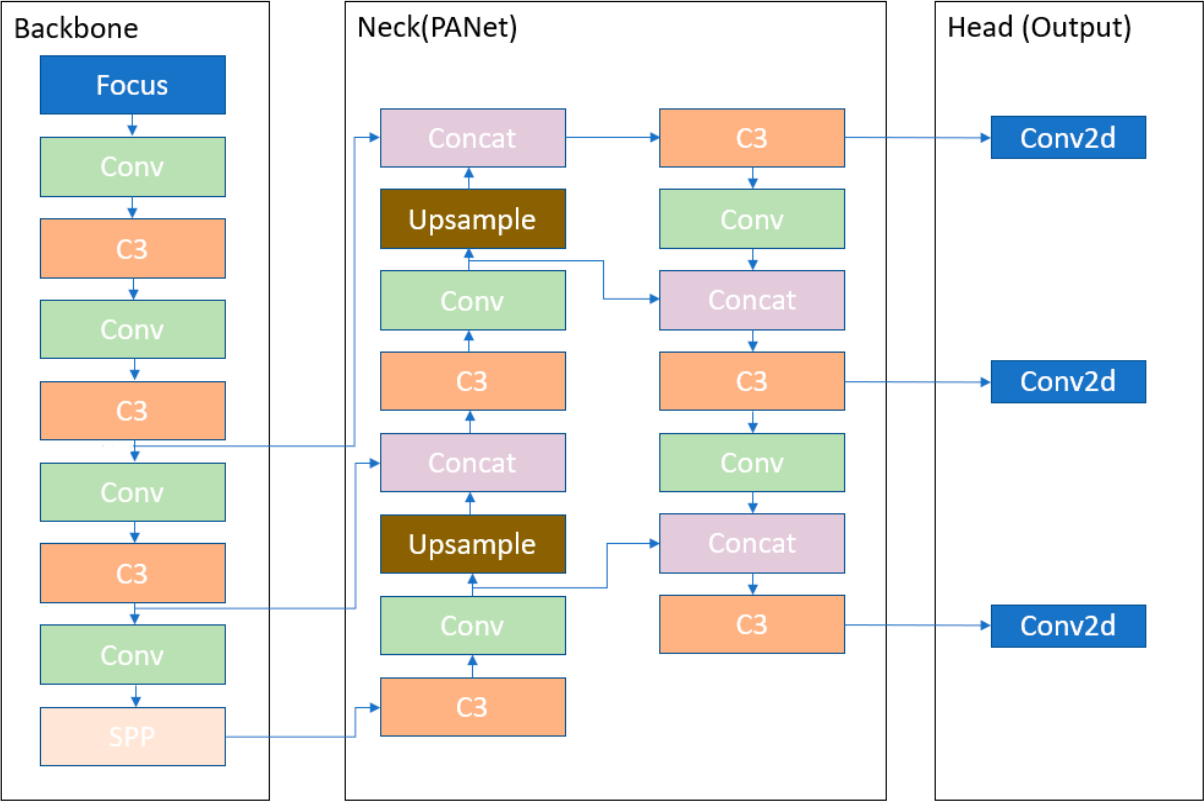
\includegraphics[width=0.95\textwidth]{Figuras/yolov5.png}
    \caption[Arquitectura de la red YOLOv5.]{Arquitectura de la red YOLOv5. Fuente: \cite{nepal-2022}.}
    \label{fig:yolov5}
\end{figure}


En \cite{nepal-2022} se indica que la arquitectura YOLOv5, al entrenarse sobre el conjunto de datos denominado DOTA (conjunto de imágenes aéreas), alcanza una precisión de 0.707 y un F1 Score de 0.655 en la tarea de reconocer y ubicar objetos en imágenes. En \cite{ahmad-2022}, se trabajó con esta arquitectura y se entrenó con un conjunto de datos de 7046 imágenes de insectos tomadas de internet (algunos ejemplos pueden verse en la Figura \ref{fig:yolov5-insects}). De igual manera, ser enfocó en la tarea de reconocer insectos en una imagen, en este caso, se obtuvo una precisión de entre el 0.7453 y el 0.9450 (con variaciones menores en la arquitectura); por el lado del F1 Score, se obtuvo entre 0.77 y 0.96. Por otro lado, en \cite{qi-2023}, se utilizó un conjunto de 25028 imágenes obtenidas por los autores del estudio; se obtuvo una precisión de 0.927 y un F1 Score de 0.932.

\begin{figure}[ht]
    \centering
    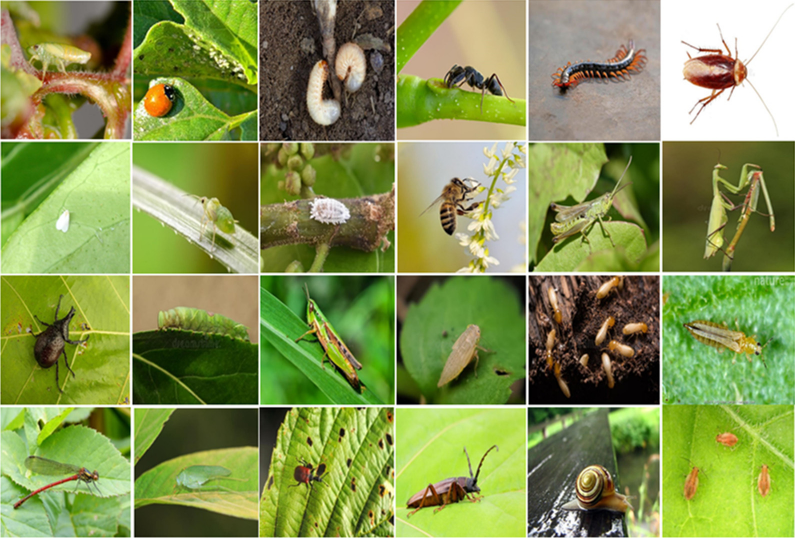
\includegraphics[width=0.95\textwidth]{Figuras/yolov5-insects.png}
    \caption[Ejemplos de imágenes de insectos utilizadas en {[6]}.]{Ejemplos de imágenes de insectos utilizadas en \cite{ahmad-2022}. Fuente: \cite{ahmad-2022}.}
    \label{fig:yolov5-insects}
\end{figure}

\subsection{EfficientNet}

EfficientNet \cite{tan-2019} es una arquitectura de red neuronal convolucional que se caracteriza por ser eficiente en términos de cómputo y parámetros. El modelo toma como entradas las imágenes y produce como salida la clasificación de objetos en la imagen, de manera específica: clase del objeto identificado y nivel de confianza. Cabe indicar que, a diferencia de YOLOv5, este modelo no realiza la localización del objeto.

En la Figura \ref{fig:efficientnet} se presenta la arquitectura de la red. Se aprecia que esta red tiene una estructura simple, pues es una capa convolucional (\texttt{Conv}), seguida de múltiples capas \texttt{MBconv} (capa convolucional móvil con cuello de botella invertido \cite{sandler2019}). A cada una de estas capas se aplicó una optimización «apretar y excitar» que tiene el objetivo de mejorar la capacidad de atención de la red, lo cual implica un incremento en la capacidad de discriminación de la información de la imagen.

\begin{figure}[ht]
    \centering
    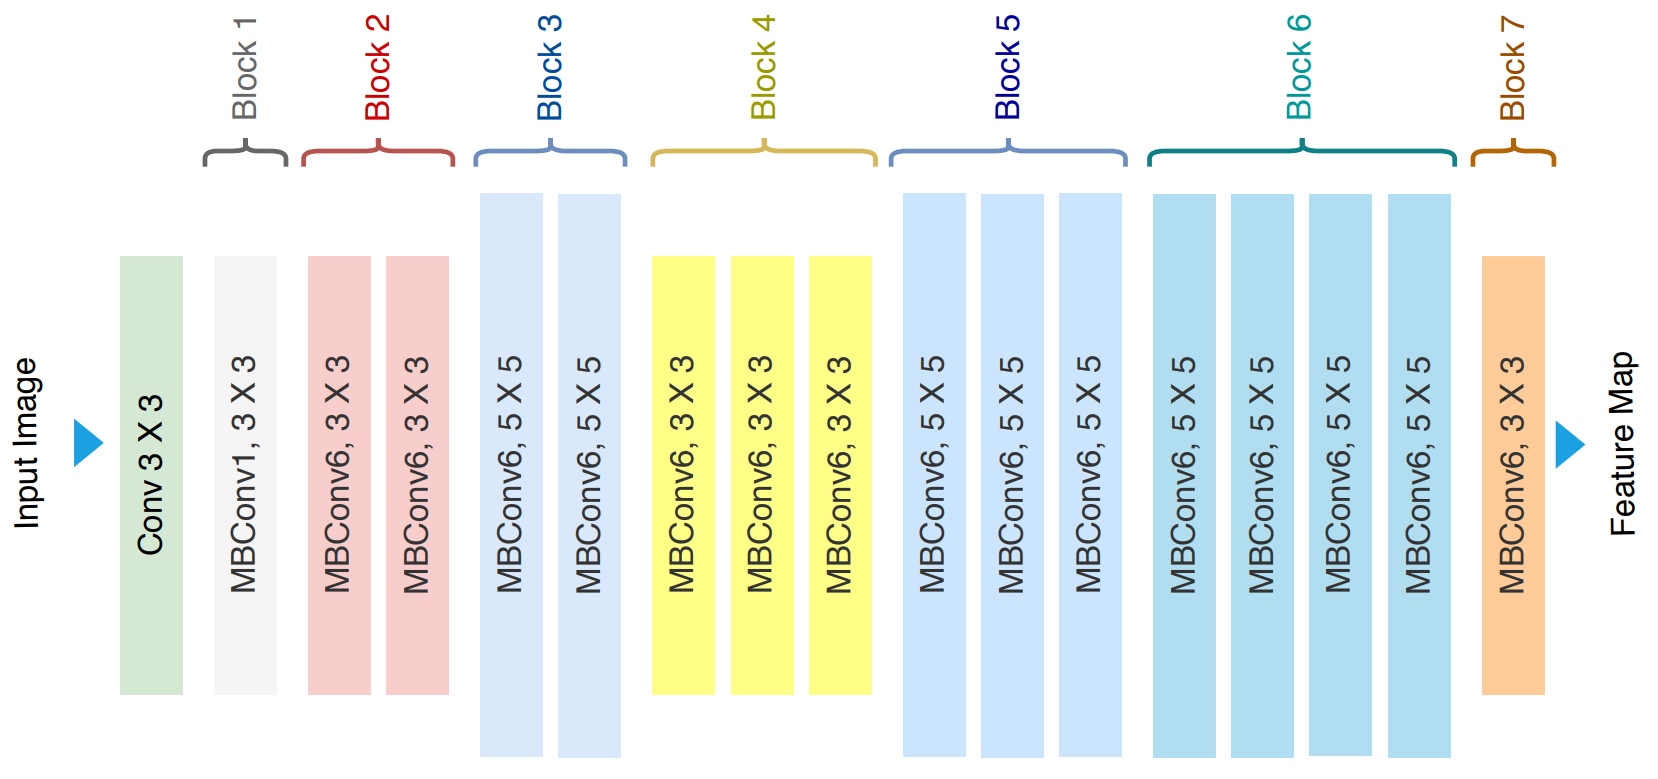
\includegraphics[width=0.95\textwidth]{Figuras/efficientnet.png}
    \caption[Arquitectura de la red EfficientNet.]{Arquitectura de la red EfficientNet. Fuente: \cite{ahmed2021}.}
    \label{fig:efficientnet}
\end{figure}

Inicialmente, esta red se entrenó usando el conjunto de datos ImageNet, donde obtuvo una precisión de 0.933 (el artículo no especifica el F1 score alcanzado) \cite{tan-2019} en la tarea de reconocimiento de objetos en imágenes. Adicionalmente, el artículo destaca que esta precisión es alcanzada entre 5.7 y 6.1 veces más rápido que otras arquitecturas, como ResNet.

En \cite{bjerge-2023}, se utilizó esta red con un conjunto de datos de 1622 imágenes de insectos. Estas imágenes fueron tomadas de \cite{XIE2015123}, donde se tenían 24 especies diferentes de insectos (algunos ejemplos pueden verse en la Figura \ref{fig:efficientnet-insects}). Se obtuvo una precisión de entre 0.9095 y 0.9751 (dependiendo de la cantidad de clases utilizadas).

\begin{figure}[ht]
    \centering
    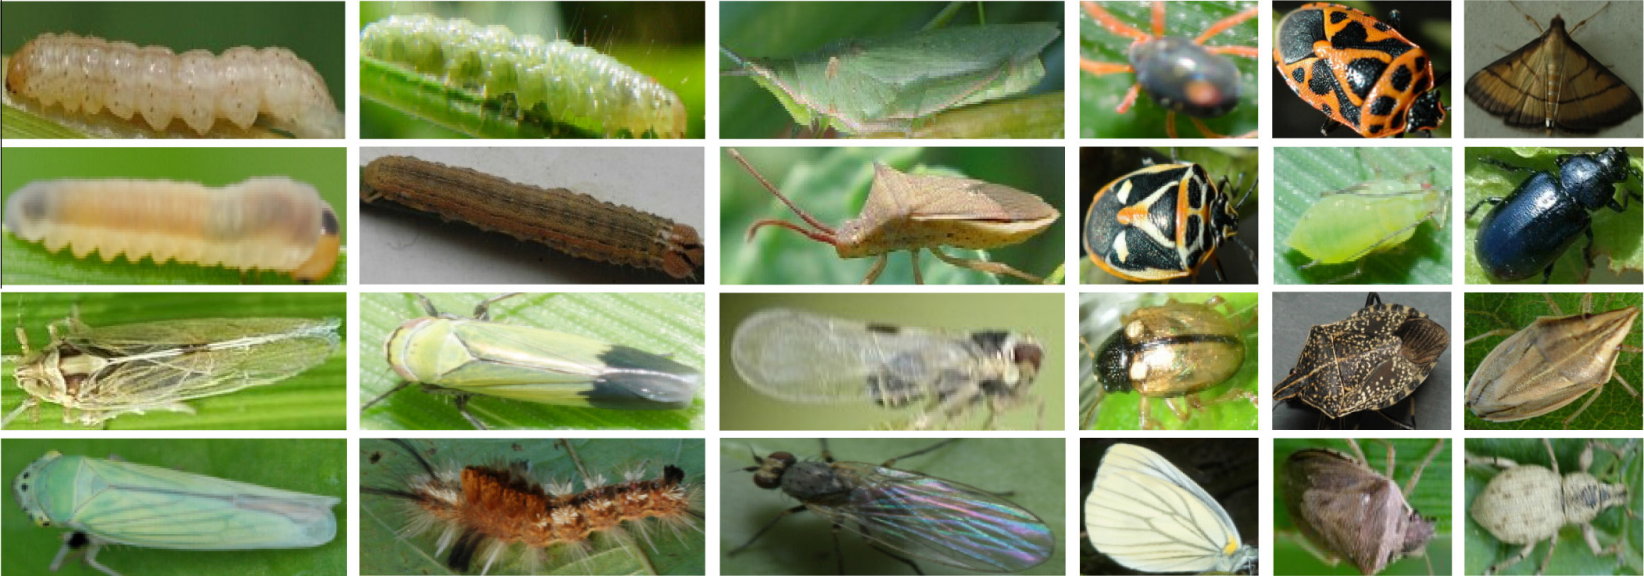
\includegraphics[width=0.95\textwidth]{Figuras/efficientnet-insects.png}
    \caption[Ejemplos de imágenes de insectos utilizadas en {[20]}.]{Ejemplos de imágenes de insectos utilizadas en \cite{bjerge-2023}. Fuente: \cite{bjerge-2023}.}
    \label{fig:efficientnet-insects}
\end{figure}

\subsection{Otras arquitecturas}

Cabe indicar que, YOLOv5 y EfficientNet no son las únicas arquitecturas que han sido sometidas a conjuntos específicos de insectos. En \cite{li-2021} se cuenta con un análisis detallado de modelos usados en la detección de insectos en imágenes. En la Tabla \ref{table:arquitecturas} se presenta un resumen de los resultados obtenidos con los modelos más relevantes.

\begin{table}[H]

\centering\small
\begin{tabular}{@{}lrrr@{}}
\toprule
    \textbf{Modelo} & \textbf{Imágenes} & \textbf{Categorías} & \textbf{Precisión}
\\ \midrule
    Small-sample learning \cite{yang-2021}& 11000 & 220 & 0.5765\\
    Tiny YOLOv3 \cite{rustia-2021} & 400 & 5 & 0.9800\\
    Fine-tuned ResNet-50 \cite{malathi-2021}& 3549 & 10 & 0.9501\\
    Ensemble CNNs \cite{khanramaki-2021}& 1774 & 3 & 0.9904\\
    EfficientNet-B6 \cite{sagar-2020} & 170000 & 1300 & 0.8650\\
    GoogLeNet \cite{li-2020} & 5629 & 10 & 0.9461\\
    ResNet-101 \cite{cheng-2017}& 550 & 10 & 0.9867\\
    AlexNet \cite{liu-2016}& 5000 & 12 & 0.9510\\
\bottomrule
\end{tabular}
\caption[Arquitecturas utilizadas en la detección de insectos en imágenes.]{Resumen de arquitecturas utilizadas en la detección de insectos en imágenes. Fuente \cite{li-2021}.}
\label{table:arquitecturas}
\end{table}

\subsection{Posibles dificultades}

Li, et al. \cite{li-2021} indican que, a pesar de que los modelos de detección de objetos en imágenes presenta buenos resultados, en el caso de realizar reconocimiento de insectos sobre plantas, se pueden presentar algunas dificultades. Las más relevantes para este trabajo son: la complejidad del fondo de la imagen, los diversos tamaños de los insectos y el desbalance de clases. Con respecto a los dos primeros problemas, se tiene que arquitecturas de la familia YOLO presentan buenos resultados en este aspecto \cite{he-2020}.

Para solventar el desbalance de clases, se aplicarán técnicas de aumento de datos (\textit{data augmentation}), las mismas que serán descritas en la siguiente sección.

\section{Preprocesamiento de imágenes}

Dado un conjunto de imágenes, el primer paso es realizar un preprocesamiento de las mismas antes de ser utilizadas en un modelo. Este preprocesamiento va desde el etiquetado hasta el aumento de datos.

A pesar de los múltiples conjuntos de datos sobre insectos (ver \cite{li-2021}, Tabla~3), en este trabajo se usará un conjunto de datos propio. Por lo tanto, se debe realizar el etiquetado de las imágenes; para esto, existen herramientas como \textit{LabelImg} \cite{LabelImg}, orientadas tanto al etiquetado de objetos como a su localización.

Posteriormente, se debe realizar una redimensión de las imágenes, de tal manera que todas tengan el mismo tamaño. Esto es necesario para que el modelo pueda procesar las imágenes de manera eficiente. A continuación, para solventar problemas de limitación de variedad de clases y localizaciones, se puede realizar un aumento de datos, el cual consiste en generar nuevas imágenes a partir de las imágenes originales. Para esto, se pueden utilizar técnicas como el volteo horizontal y vertical, el recorte de imágenes, el cambio de brillo, entre otras. Adicionalmente, al tratarse de imágenes de insectos, es usual que no se tenga un enfoque apropiado en el objetivo, para solventar esto, a partir de imágenes con enfoque adecuado, se puede agregar ruido Gaussiano para simular el desenfoque \cite{khanramaki-2021}.


\section{Redes de polinización}

Las redes de polinización son redes de interacción entre especies de plantas y polinizadores. Contar con este tipo de redes de un determinado ecosistema es esencial para entender la dinámica de las interacciones entre las especies, lo cual es importante para la estabilidad de los ecosistemas y, por ende, para la conservación de la biodiversidad.

Estas redes tradicionalmente se construyen mediante observación y trabajo de campo que normalmente son incompletos y, por esto, hace falta aplicar técnicas estadísticas. Para esto, se puede utilizar la metodología propuesta por Young et al. \cite{young-2021}, la cual se resume a continuación.

Se consideran $n_p$ especies de plantas y $n_a$ especies de polinizadores, se tiene la matriz $M = (M_{ij})$, de orden $n_p\times n_a$, donde $M_{ij}$ es el número de veces que se ha detectado una interacción de la especie $j$ con la planta $i$. Se tiene que $M$ podría representar un grafo bipartito ponderado (matriz de incidencia). El objetivo es, a partir de este grafo, generar otro donde se tenga una arista de un polinizador a una planta si el polinizador prefiere a dicha planta; a la representación matricial de este grafo se la denomina $B$. De esta manera, se tiene que $B_{ij}$ es igual a $1$ si la especie $j$ es un polinizador de la planta $i$ y $0$ en caso contrario.

Con esto, Young et al. \cite{young-2021} proponen que $B_{ij}$ representa una variable aleatoria de la cual, al tener la matriz $M$, se puede calcular su probabilidad condicional. Para esto, deducen que
\[
    P(B_{ij}=1|M) = \sum_{B} \int B_{ij} P(B, \theta|M)\, d\theta
\]
donde la suma corre sobre todas las posibles matrices de incidencia y $\theta$ representa todos los parámetros del modelo planteado: cambio al número promedio de visitas ($r$), el efecto del muestreo ($C$) y abundancia de plantas ($\sigma$) e insectos ($\tau$). A pesar de que, con este enfoque, se tiene una distribución de probabilidad para $B$, esta no es computacionalmente efectiva, por lo tanto, se puede utilizar técnicas de Monte Carlo para aproximar la distribución de probabilidad.

Para esto, se tiene que el número de visitas $M_{ij}$ es una variable aleatoria de Poisson con media
\[
    \mu_{ij} = C \sigma_i \tau_j (1 + rB_{ij}).
\]
De esta manera, si se considera que la probabilidad de que un insecto sea polinizador de una planta como una variable uniforme de probabilidad $\rho$, se tiene que
\[
    P(B, \theta|M) \propto P(\theta) \prod_{ij} (1-\rho)^{1-B_{ij}} \rho^{B_{ij}}  \frac{\mu_{ij}^{M_{ij}} }{M_{ij}!}e^{-\mu_{ij}} .
\]
Con esto, se puede utilizar un algoritmo de maximización de la esperanza para obtener los parámetros del modelo y, de esta manera, obtener la distribución de probabilidad de $B$.


Esta metodología proporcionó resultados coherentes con las propiedades de la distribución de conexión que fue propuesta como un invariante en este tipo de redes en \cite{jordano-2002}.
\chapter{Implementación del trabajo}
\label{chapter:implementacion}

Durante el desarrollo de este trabajo, se ha seguido un ciclo de trabajo iterativo, en el que se han ido realizando pruebas y modificaciones sobre el código, hasta obtener los resultados deseados. En este capítulo se describirán los pasos seguidos para la implementación del trabajo, así como las herramientas utilizadas para ello. Este proceso se puede dividir en las siguientes etapas:
\begin{itemize}
    \item \textbf{Preprocesamiento de datos:} en esta etapa se ha realizado manipulación y limpieza de datos, de tal forma que estos se encuentren en un formato adecuado para ser procesados por los modelos. A la par, se ha realizado un análisis exploratorio de los datos, con el fin de obtener información relevante sobre los mismos.
    \item \textbf{Aplicación de un modelo basado en YOLOv5}: en esta etapa se ha entrenado modelo basado en YOLOv5, con el fin de realizar la detección de insectos en las imágenes.
    \item \textbf{Aplicación de un modelo basado en EfficientNet}: en esta etapa se hace lo análogo a la etapa anterior, pero con un modelo basado en EfficientNet.
    \item \textbf{Evaluación de los modelos:} en esta etapa se evalúan los modelos, con el fin de determinar cuál de ellos es el más adecuado para el problema.
    \item \textbf{Reconstrucción de red de polinizadores:} en esta etapa, utilizando el modelo seleccionado, se reconstruye la red de polinizadores.
\end{itemize}

\section{Entorno de trabajo}

En general, se utilizó el lenguaje de programación Python para el desarrollo de este trabajo. En específico, se desarrolló el código en el entorno Jupyter Notebook. Para el modelo basado en YOLOv5, se utilizó la librería \textit{Pytorch}, mientras que para el modelo basado en EfficientNet, se utilizó la librería \textit{Tensorflow}. Finalmente, para la reconstrucción, análisis y visualización de la red de polinizadores, se utilizó la librería \textit{NetworkX}.

En cuanto al hardware utilizado, se emplearon dos instancias. Para el procesamiento de datos y el entrenamiento del modelo basado en EfficientNet, se utilizó un computador de escritorio con procesador AMD Rayzen 7 de 8 núcleos y 40 GB de memoria RAM, adicionalmente, se utilizó una tarjeta gráfica NVIDIA GeForce RTX 3060 de 12 GB de memoria dedicada. Sin embargo, esto no fue suficiente para los modelos basados en YOLOv5, por lo cual se utilizó Google Colab, con una GPU Nvidia A100 de 40 GB de memoria dedicada.


\section{Procesamiento de datos}


Los datos para este estudio se obtuvieron mediante un sistema de monitoreo automático desarrollado en \cite{serra-2022}, que consistió en un ensamblaje de cámara controlado por un ordenador de placa única, específicamente una Raspberry Pi 4. Esta configuración fue elegida por su óptima resolución óptica para objetos pequeños como insectos y flores, y su capacidad para programar ciclos de vídeo en el campo. El sistema incluía una cámara Module V2 de 5MP, que proporcionaba videos de 1080p a 30 fotogramas por segundo. Para la autonomía, se utilizó una batería portátil de 1000mAh Li-polímero, que permitía hasta seis horas de funcionamiento, y los videos se almacenaban en un USB de 32 GB. Todo el conjunto estaba protegido por una caja de plástico y montado en un trípode, diseñado para registrar interacciones planta-polinizador.

Para la recopilación de datos, se programó la Raspberry Pi 4 para automatizar la grabación de videos en ciclos de 10 minutos durante periodos de una hora y media, usando un archivo '.ssh' y Python 3.0. Además de los videos capturados por este sistema, se desarrolló una biblioteca fotográfica de 12000 imágenes de insectos polinizadores. Los objetos en los fotogramas de los videos se etiquetaron manualmente utilizando el programa LabelImg.

De manera específica, para este proyecto, se seleccionó 5445 imágenes de flores con polinizadores, las cuales fueron seleccionadas por el autor de \cite{serra-2022} como las de mejor calidad. Estas imágenes contaban con diferentes dimensiones, siendo mayoritario el tamaño de 1280$\times$962 píxeles. El ancho de las imágenes era fijo, y la distribución del alto de las imágenes, en escala logarítmica, se puede apreciar en la Figura~\ref{fig:dimensiones}.

\begin{figure}[H]
    \centering
    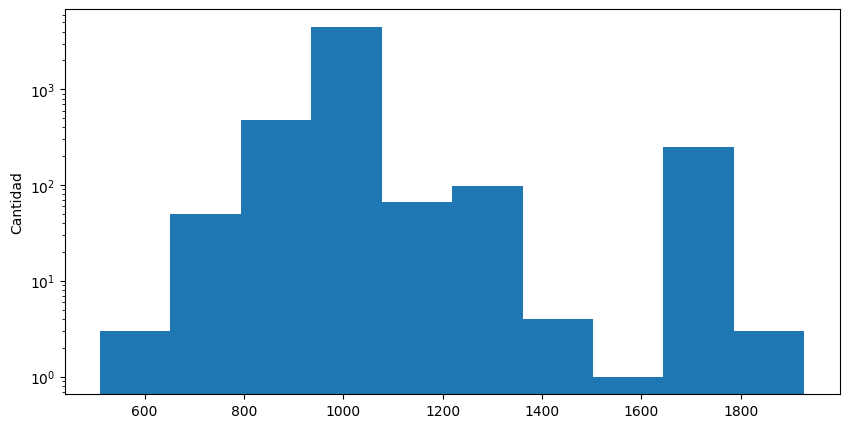
\includegraphics[width=0.8\textwidth]{Figuras/dimensiones.png}
    \caption{Distribución del alto de las imágenes, en escala logarítmica.}
    \label{fig:dimensiones}
\end{figure}

Dado que los modelos a utilizarse trabajan con imágenes del mismo tamaño, se debe estandarizar los altos de las imágenes. Para esto, se tomó como medida estándar la moda de las alturas. En las imágenes con un alto menor a este valor, se completó con un fondo blanco, mientras que en las que poseían un alto mayor a esto, se las recortó.

De cada imagen se contaba con un archivo XML, que contenía la información de las coordenadas de los polinizadores en la imagen, así como la especie de cada uno de ellos. Un ejemplo de este archivo se puede apreciar en el Código~\ref{code:xml}.

\begin{lstlisting}[language=XML, caption={Ejemplo de archivo XML de información de imágenes.}, label={code:xml}]
    <annotation>
	<folder>fotos transformades</folder>
	<filename>P1050344.JPG</filename>
	<path>F:\polinitzadors\fotos insectes\fotos transformades\P1050344.JPG</path>
	<source>
		<database>Unknown</database>
	</source>
	<size>
		<width>1280</width>
		<height>960</height>
		<depth>3</depth>
	</size>
	<segmented>0</segmented>
	<object>
		<name>Bee</name>
		<pose>Unspecified</pose>
		<truncated>0</truncated>
		<difficult>0</difficult>
		<bndbox>
			<xmin>344</xmin>
			<ymin>243</ymin>
			<xmax>569</xmax>
			<ymax>429</ymax>
		</bndbox>
	</object>
</annotation>
\end{lstlisting}

De la información de las imágenes se tomó el nombre de la imagen (\texttt{filename}), el nombre del objeto (\texttt{object, name}) y la posición (\texttt{object, bndbox}). A partir del nombre del objeto, se realizó una clasificación de los polinizadores en 7 categorías: Bee, Lepidoptera, Diptera, Coleoptera, Others, Wasp y Hoverfly. Cabe señalar que, en algunas imágenes, se encontraban más de un polinizador. En la Figura~\ref{fig:especies} se puede apreciar un ejemplo de cada una de estas categorías.

\begin{figure}[H]
    \centering
    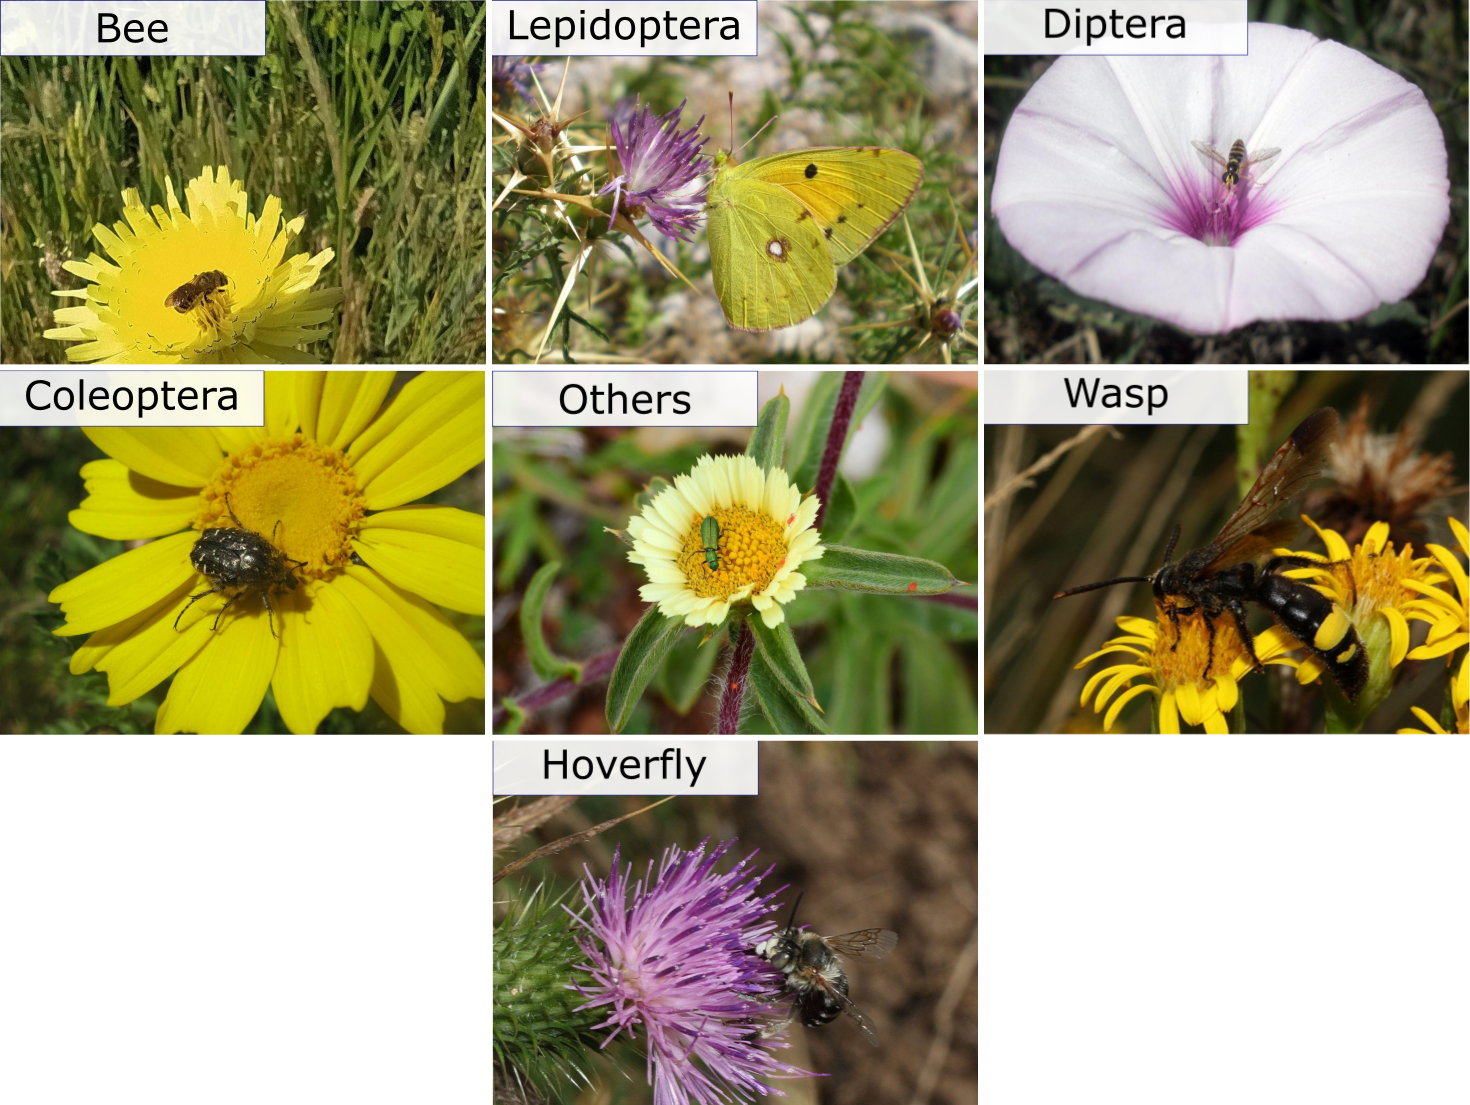
\includegraphics[width=0.95\textwidth]{Figuras/ejemplos.png}
    \caption{Ejemplo de cada una de las especies de polinizadores.}
    \label{fig:especies}
\end{figure}

La distribución de las especies, por categoría, en las imágenes se puede apreciar en la Figura~\ref{fig:distribucion_especies}, en escala logarítmica. Se observa que la especie más abundante es «Bee», con 5189, seguida de «Lepidoptera», con 510, y «Diptera», con 305. Por otro lado, las especies menos abundantes son «Wasp», con 109, y «Hoverfly», con 81. En total, en las 5445 imágenes se tienen 6681 polinizadores, por lo cual, para el modelo, se tiene en la práctica 6681 imágenes etiquetadas.

\begin{figure}[H]
    \centering
    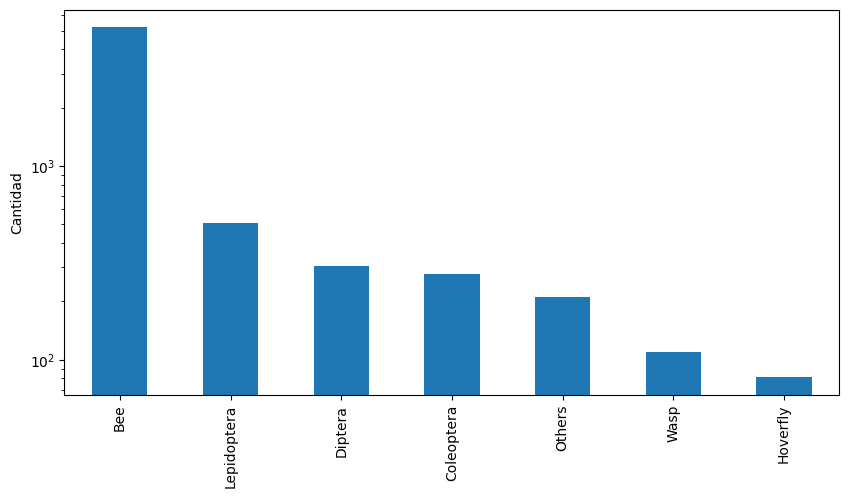
\includegraphics[width=0.79\textwidth]{Figuras/distribucion_especies.png}
    \caption{Distribución de las especies en las imágenes, en escala logarítmica.}
    \label{fig:distribucion_especies}
\end{figure}

Dada la abundante cantidad de imágenes de la especie «Bee», se decidió realizar un submuestreo de estas imágenes, con el fin de balancear la cantidad de imágenes de cada especie. Para ello, se descartaron, mediante inspección directa, imágenes similares, de una misma planta, que contenga la especie «Bee» o «Lepidoptera». El resultado de este proceso se puede apreciar en la Figura~\ref{fig:submuestreo}. De esta manera, el conjunto de datos con el que se trabajará cuenta con 2121 imágenes.

\begin{figure}[H]
    \centering
    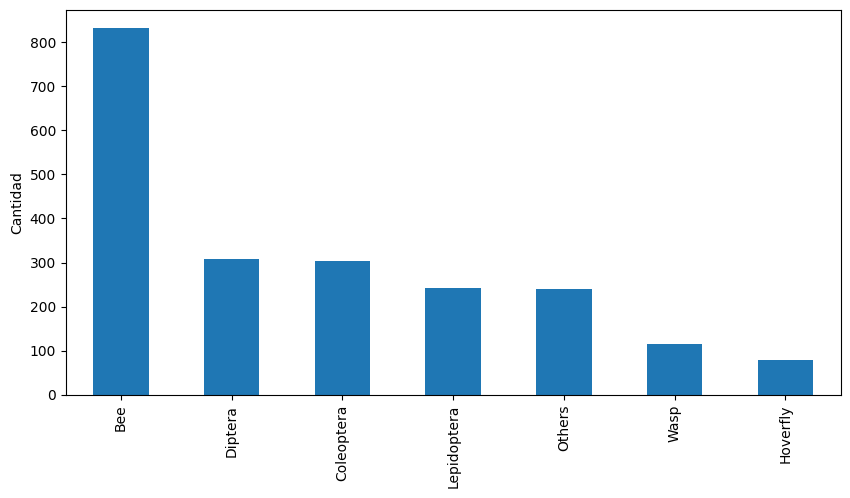
\includegraphics[width=0.79\textwidth]{Figuras/submuestreo.png}
    \caption{Submuestreo de imágenes de la categoría «Bee» y «Lepidoptera».}
    \label{fig:submuestreo}
\end{figure}


\subsection{Aumento de datos}


Para el aumento de datos, se procedió a realizar reflexiones. En las dos clases menos abundantes, «Wasp» y «Hoverfly», se realizó reflexión horizontal y vertical, mientras que en las demás clases, salvo «Bee», se realizó reflexión horizontal. En la Figura~\ref{fig:reflexiones} se puede apreciar un ejemplo de este proceso.

\begin{figure}[H]
    \centering
    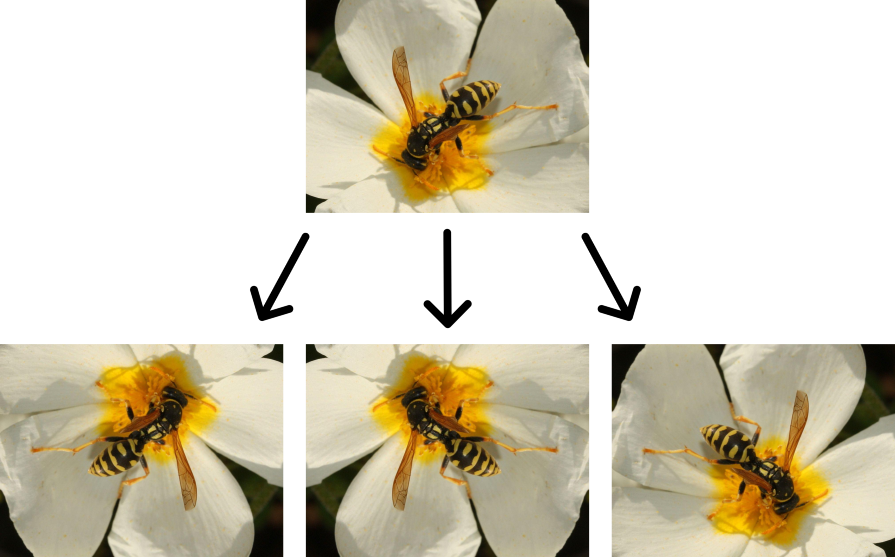
\includegraphics[width=0.75\textwidth]{Figuras/reflexion.png}
    \caption{Ejemplo de reflexiones realizadas.}
    \label{fig:reflexiones}
\end{figure}

Con esto, se obtuvieron 3415 imágenes y se mejoró la distribución de las mismas en las diferentes categorías. Esta distribución se puede apreciar en la Figura~\ref{fig:distribucion_especies_aumento}.

\begin{figure}[H]
    \centering
    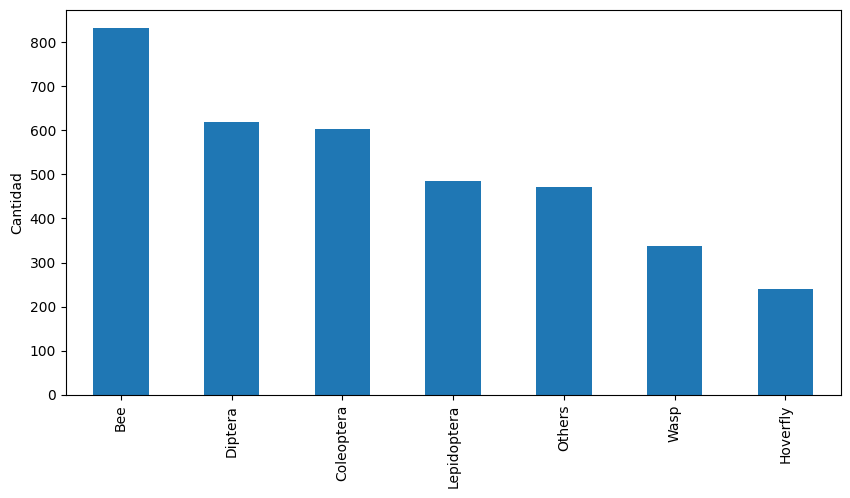
\includegraphics[width=0.8\textwidth]{Figuras/distribucion_especies_aumento.png}
    \caption{Distribución de las especies en las imágenes luego del aumento de datos.}
    \label{fig:distribucion_especies_aumento}
\end{figure}

Con estos resultados, se dividió los datos en los conjuntos de entrenamiento, validación y prueba. La distribución de los datos en estos conjuntos muestra en la Tabla~\ref{tab:distribucion_conjuntos}.

\begin{table}[H]
    \centering\small
    \begin{tabular}{cccc}
        \toprule
         & \textbf{Entrenamiento} & \textbf{Validación} & \textbf{Prueba} \\
        \midrule
        {Bee} 
        & 184 & 46 & 581 \\
        {Lepidoptera} 
        & 184 & 46 & 364 \\
        {Diptera} 
        & 184 & 46 & 322 \\
        {Coleoptera} 
        & 184 & 46 & 240 \\
        {Others} 
        & 184 & 46 & 191 \\
        {Wasp} 
        & 184 & 46 & 97 \\
        {Hoverfly} 
        & 184 & 46 & 10 \\
        \midrule
        \textbf{Total}
        & 1288 & 322 & 1805 \\
        \bottomrule
    \end{tabular}
    \caption{Distribución de los datos en los conjuntos de entrenamiento, validación y prueba.}
    \label{tab:distribucion_conjuntos}
\end{table}

\section{Aplicación de modelos}

\subsection{YOLOv5}

Para iniciar el análisis de los modelos, se procedió a realizar una prueba con el modelo YOLOv5, con el fin de determinar si este era capaz de detectar los polinizadores en las imágenes. Para ello, se utilizó el conjunto de prueba para determinar las detecciones realizadas por el modelo; cabe recalcar que, el modelo YOLOv5 está entrenado con el conjunto COCO, el cual no cuenta con polinizadores. Por esto, se obtuvieron diversos objetos detectados, los primeros diez objetos más detectados se pueden apreciar en la Tabla~\ref{tab:objetos_detectados}.

\begin{table}[H]
    \centering\small
    \begin{tabular}{cc}
        \toprule
        \textbf{Objeto} & \textbf{Cantidad} \\
        \midrule
        no detection &  853 \\
        bird         &  322 \\
        banana       &  109 \\
        dining table &   98 \\
        apple        &   67 \\
        potted plant &   25 \\
        microwave    &   19 \\
        orange       &   19 \\
        broccoli     &   18 \\
        chair        &   16 \\
        \bottomrule
    \end{tabular}
    \caption{Objetos detectados por el modelo YOLOv5.}
    \label{tab:objetos_detectados}
\end{table}

Cabe destacar que, en las detecciones, se observan pocas referentes a plantas y ninguna referente a insectos. Adicionalmente, en los casos de detección de plantas, no se encuentran relacionados con las especies que se tienen en las imágenes.

Con este resultado base, se procedió a entrenar el modelo YOLOv5 con los datos de polinizadores. Para ello, se utilizó el conjunto de entrenamiento, y se validó con el conjunto de validación. El entrenamiento se realizó con 100 épocas, con un tamaño de lote de 32 imágenes, y con un tamaño de imagen de 1280 píxeles de ancho. 

Para evaluar el rendimiento del modelo YOLOv5 entrenado, se emplearon dos tipos de gráficos basados en el conjunto de validación: las curvas de precisión-confianza y de exhaustividad-confianza.

\begin{itemize}
    \item 
    \textbf{Curvas de Precisión-Confianza (\textit{precision-confidence}):} Estas curvas ilustran la relación entre la precisión del modelo y el nivel de confianza (o probabilidad) asignado a sus predicciones. La precisión se define como la proporción de identificaciones correctas (verdaderos positivos) entre todas las identificaciones realizadas (verdaderos positivos más falsos positivos). En este gráfico, el eje horizontal representa la confianza del modelo en sus predicciones, mientras que el eje vertical muestra la precisión correspondiente a cada nivel de confianza. Un modelo ideal tendría una curva que se mantiene alta a medida que aumenta el nivel de confianza, indicando que puede mantener una alta precisión incluso cuando está muy seguro de sus predicciones.
    \item 
    \textbf{Curvas de Exhaustividad-Confianza (\textit{recall-confidence}):} Estas curvas muestran cómo la exhaustividad (o recuperación) del modelo varía con diferentes niveles de confianza. La exhaustividad se refiere a la proporción de casos positivos reales (verdaderos positivos) que el modelo ha identificado correctamente, respecto al total de casos positivos reales (verdaderos positivos más falsos negativos). En estas curvas, el eje horizontal representa la confianza, y el eje vertical muestra la exhaustividad. Una curva ideal sería aquella que se mantenga alta en todos los niveles de confianza, lo que indica que el modelo es capaz de identificar la mayoría de los casos positivos reales incluso con un alto nivel de confianza en sus predicciones.
\end{itemize}
    
En lo que respecta a la curva de precisión-confianza (Figura~\ref{fig:P_curve}), se tiene que la precisión óptima para todas las clases se alcanza a un umbral de confianza de aproximadamente 0.948, indicando un alto grado de fiabilidad del modelo en este punto. Sin embargo, las clases individuales muestran variabilidad en la precisión; «Bee» mantienen valores altos de precisión incluso a niveles bajos de confianza, sugiriendo un reconocimiento robusto, mientras que otras clases, particularmente las agrupadas en «Others», exhiben una precisión más baja, lo que puede sugerir una mayor dificultad en su detección.

\begin{figure}[H]
    \centering
    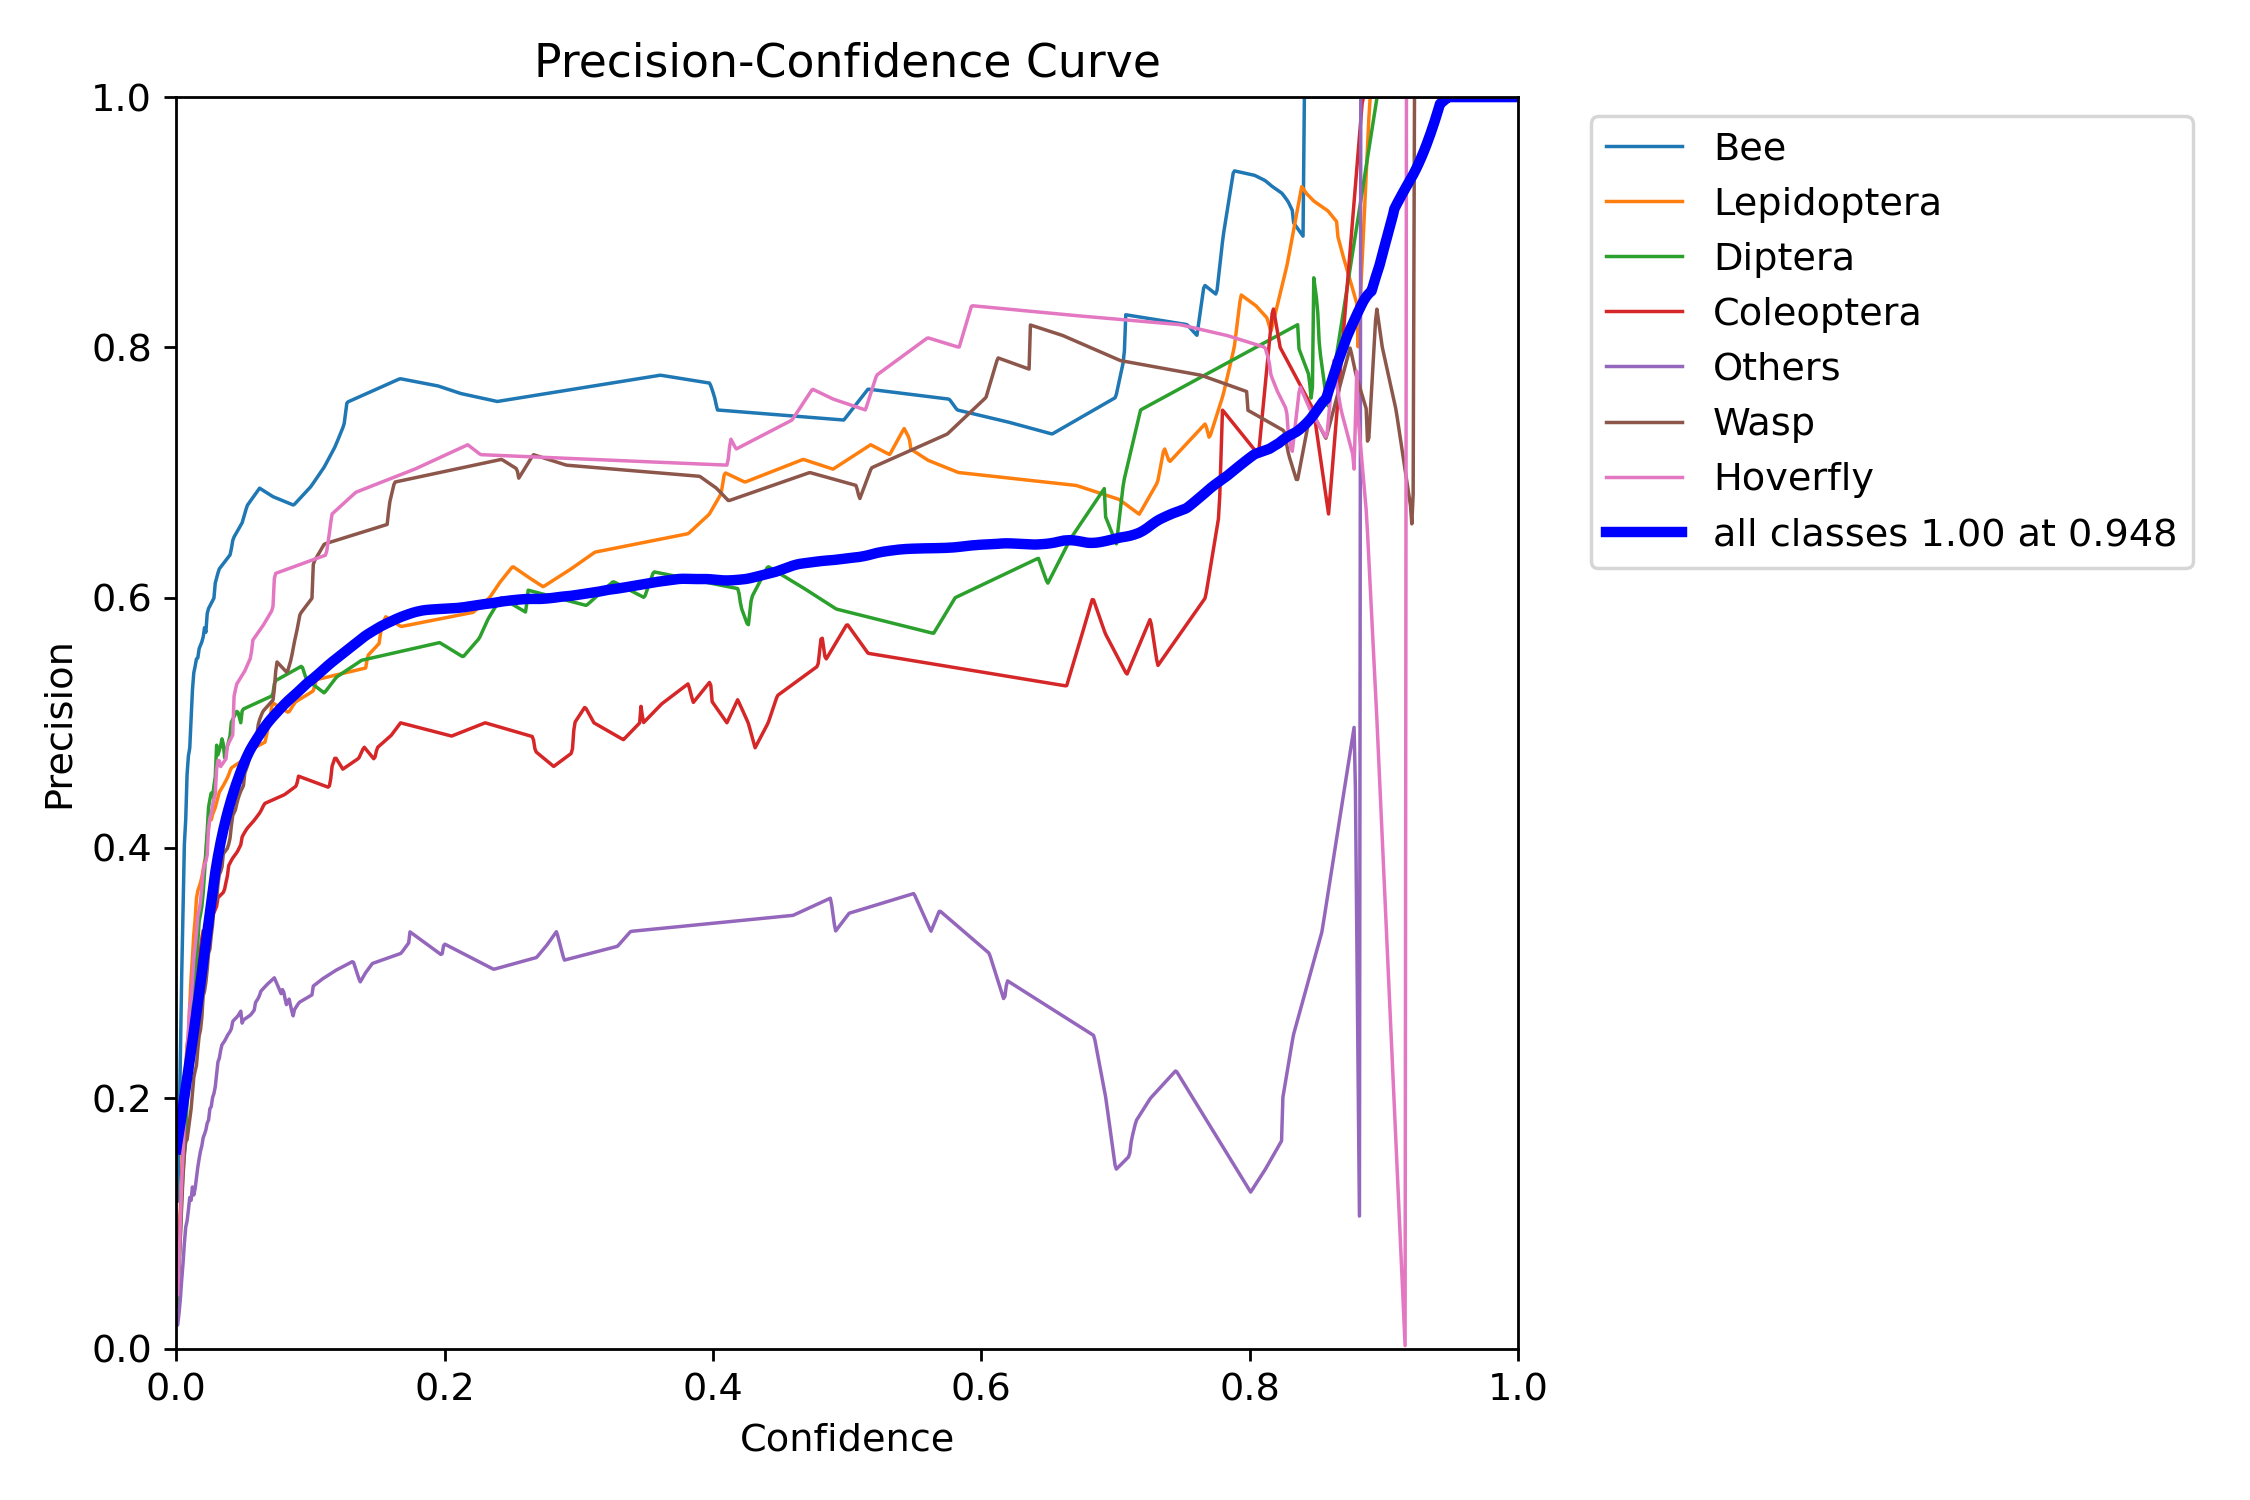
\includegraphics[width=0.85\textwidth]{Figuras/P_curve.png}
    \caption{Curvas de precisión-confianza modelo YOLOv5 en las imágenes de validación.}
    \label{fig:P_curve}
\end{figure}

\begin{figure}[H]
    \centering
    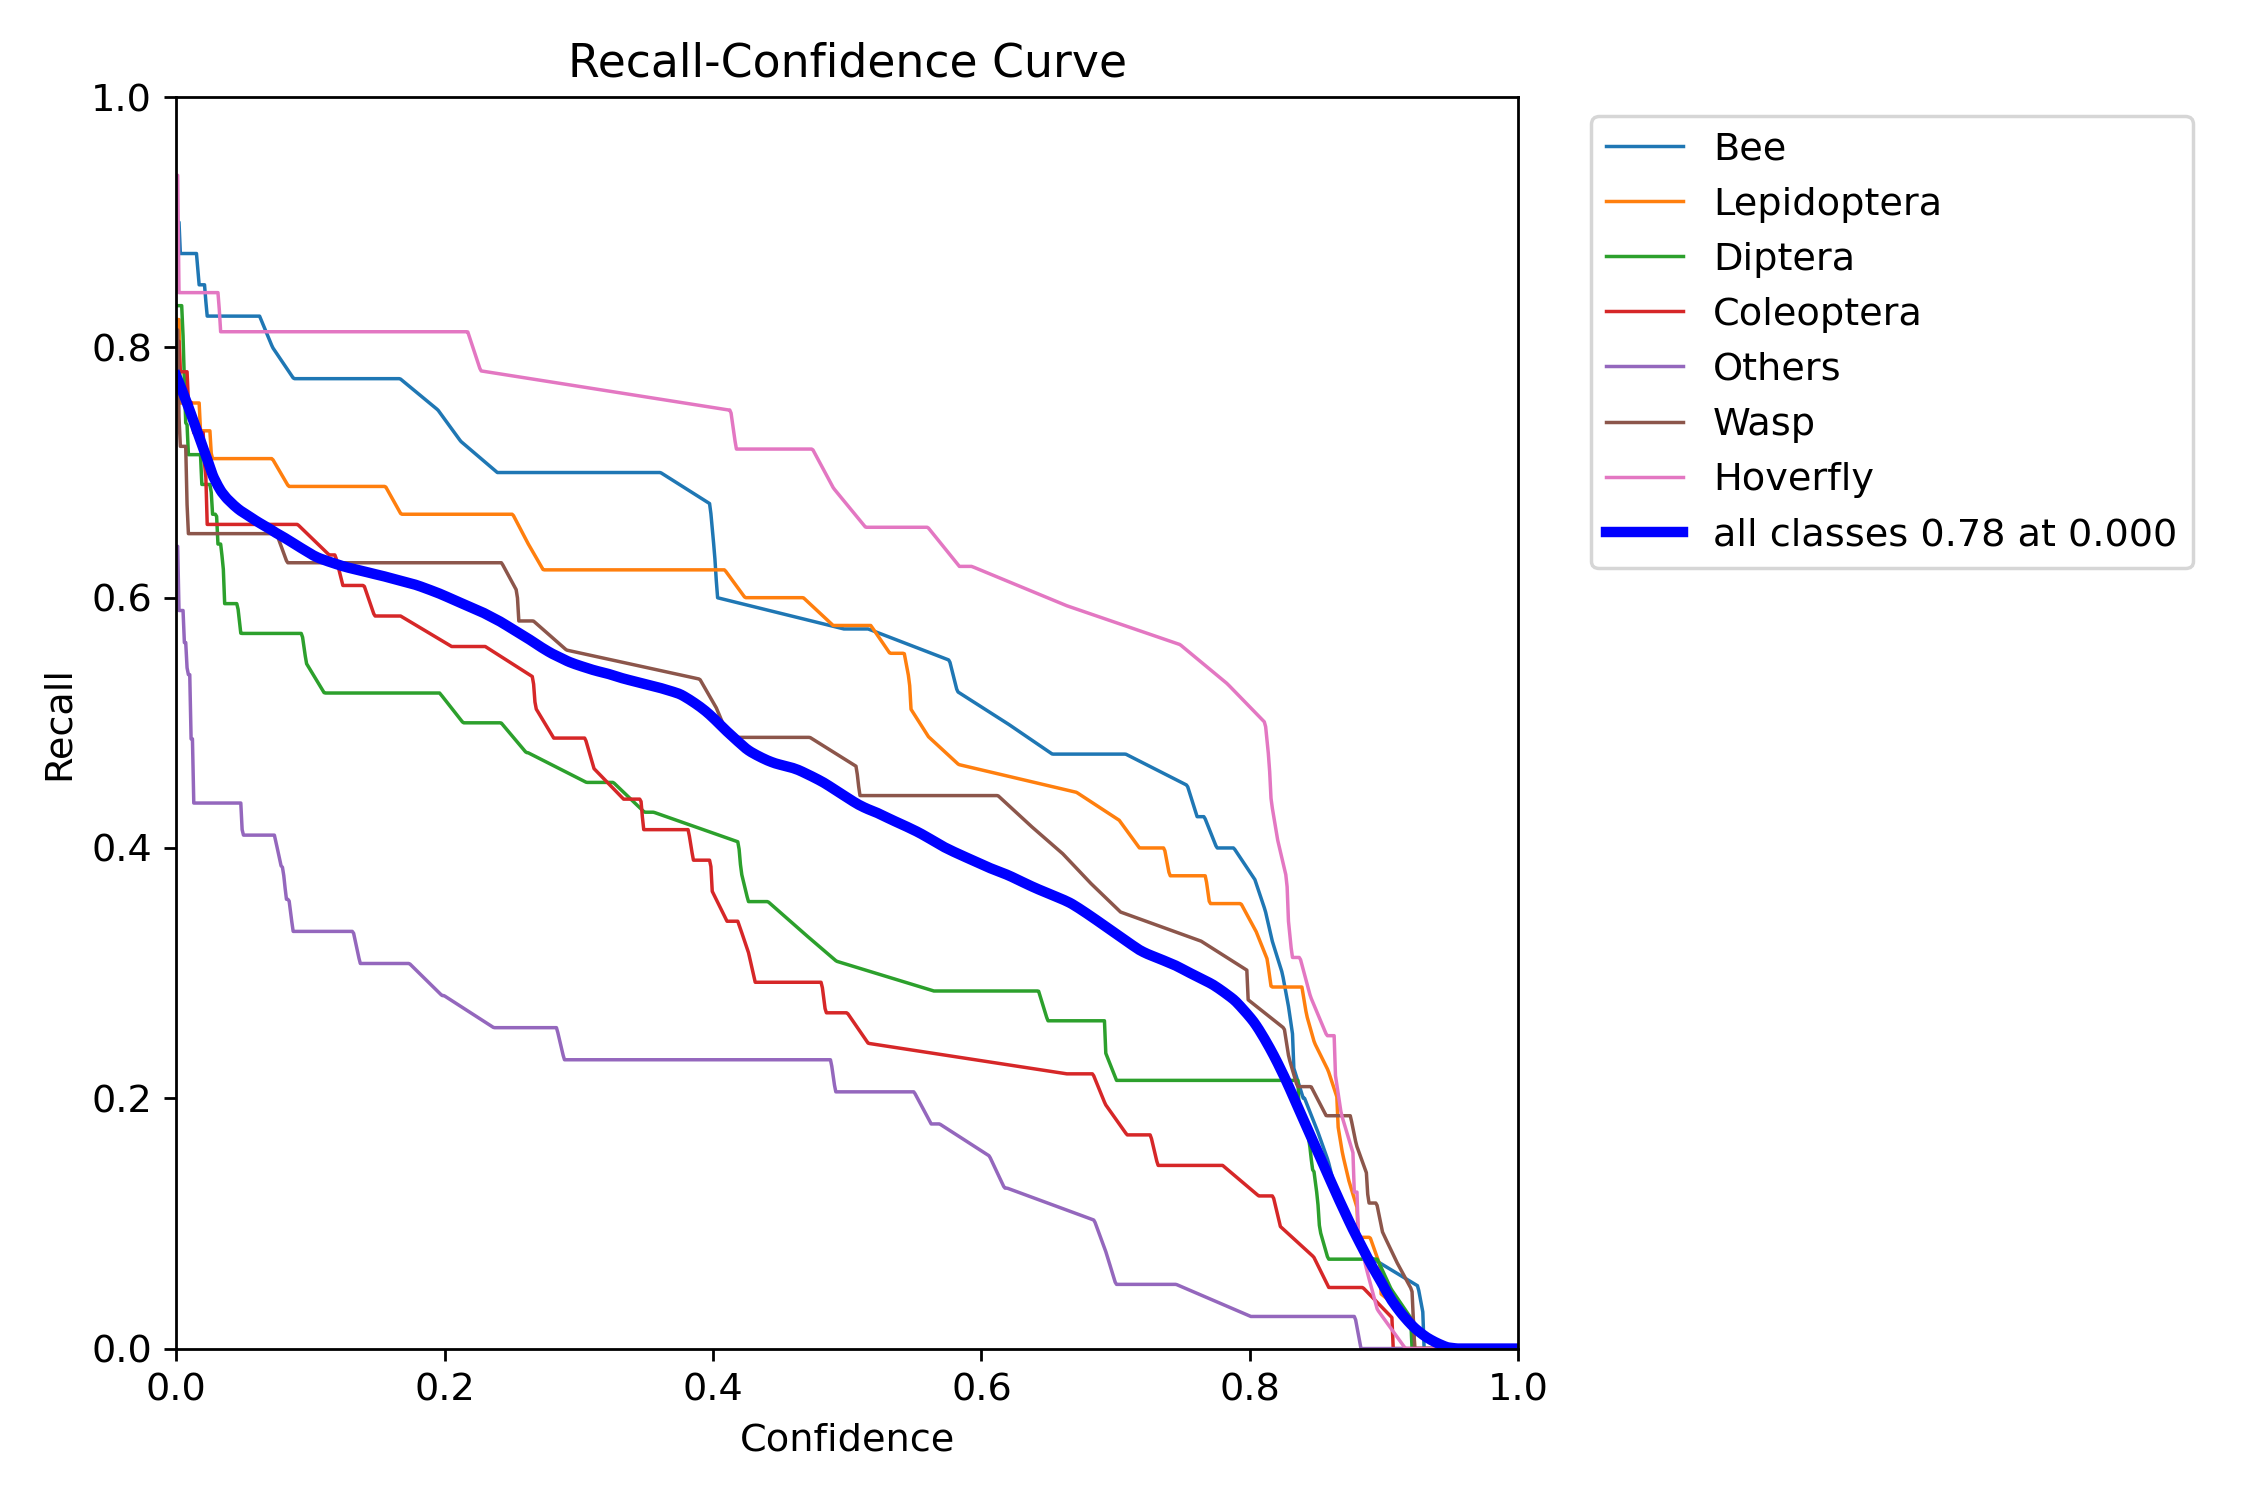
\includegraphics[width=0.85\textwidth]{Figuras/R_curve.png}
    \caption{Curvas de exhaustividad-confianza modelo YOLOv5 en las imágenes de validación.}
    \label{fig:R_curve}
\end{figure}

Por el lado de la curva exhaustividad-confianza (Figura~\ref{fig:R_curve}), demuestra que la exhaustividad general para la detección de insectos se mantiene en un nivel notable de 0.78 incluso a un umbral de confianza cero, subrayando la habilidad del modelo para detectar una gran proporción de las instancias positivas desde el inicio. Sin embargo, la exhaustividad disminuye conforme se incrementa el umbral, un comportamiento esperado al elevar la rigurosidad para la aceptación de las predicciones. Las distintas clases de insectos exhiben divergencias en la exhaustividad a lo largo de los umbrales, lo que refleja diferencias en la facilidad de detección o en la representación en el conjunto de datos.


Adicionalmente, se obtuvo la matriz de confusión con las predicciones realizadas sobre el conjunto de validación (Figura~\ref{fig:matriz_confusion_yolov5}). Se observa un alto grado de precisión en la detección de «Bee» y «Hoverlfy», con valores de 70 \% y 78 \%, respectivamente, indicando un reconocimiento efectivo de estas clases. No obstante, la confusión entre clases de insectos y el fondo, como se evidencia en los «Diptera» y «Coleoptera» mal clasificados como fondo en un 45 \% y 45 \% de los casos, respectivamente, sugiere un reto en la discriminación de características entre insectos y su entorno. Por otro lado, es remarcable el hecho de que casi no existe confusión entre las diferentes clases (valores fuera de la diagonal), llegando solo al 2 \%.

\begin{figure}[H]
    \centering
    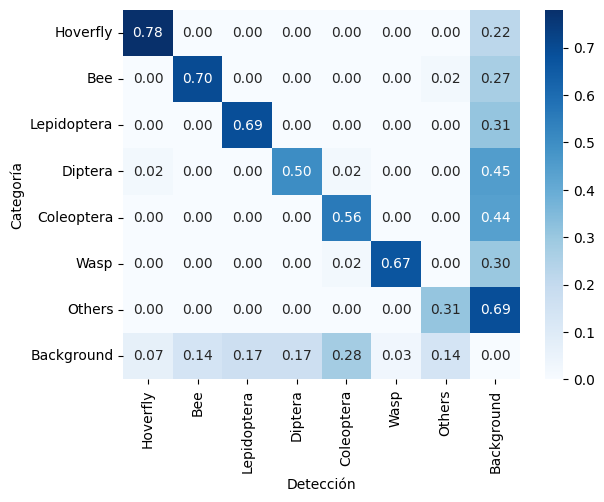
\includegraphics[width=0.75\textwidth]{Figuras/matriz_confusion_yolov5.png}
    \caption{Matriz de confusión del modelo YOLOv5.}
    \label{fig:matriz_confusion_yolov5}
\end{figure}

Por otro lado, se puede contrastar las detecciones realizadas por el modelo con las detecciones realizadas por los humanos. En la Figura~\ref{fig:comparacion_humanos_yolov5}, se puede apreciar un ejemplo de los resultados en validación. Los colores indican la clase y el valor indica la confianza de la clasificación.

\begin{figure}[H]
    \centering
    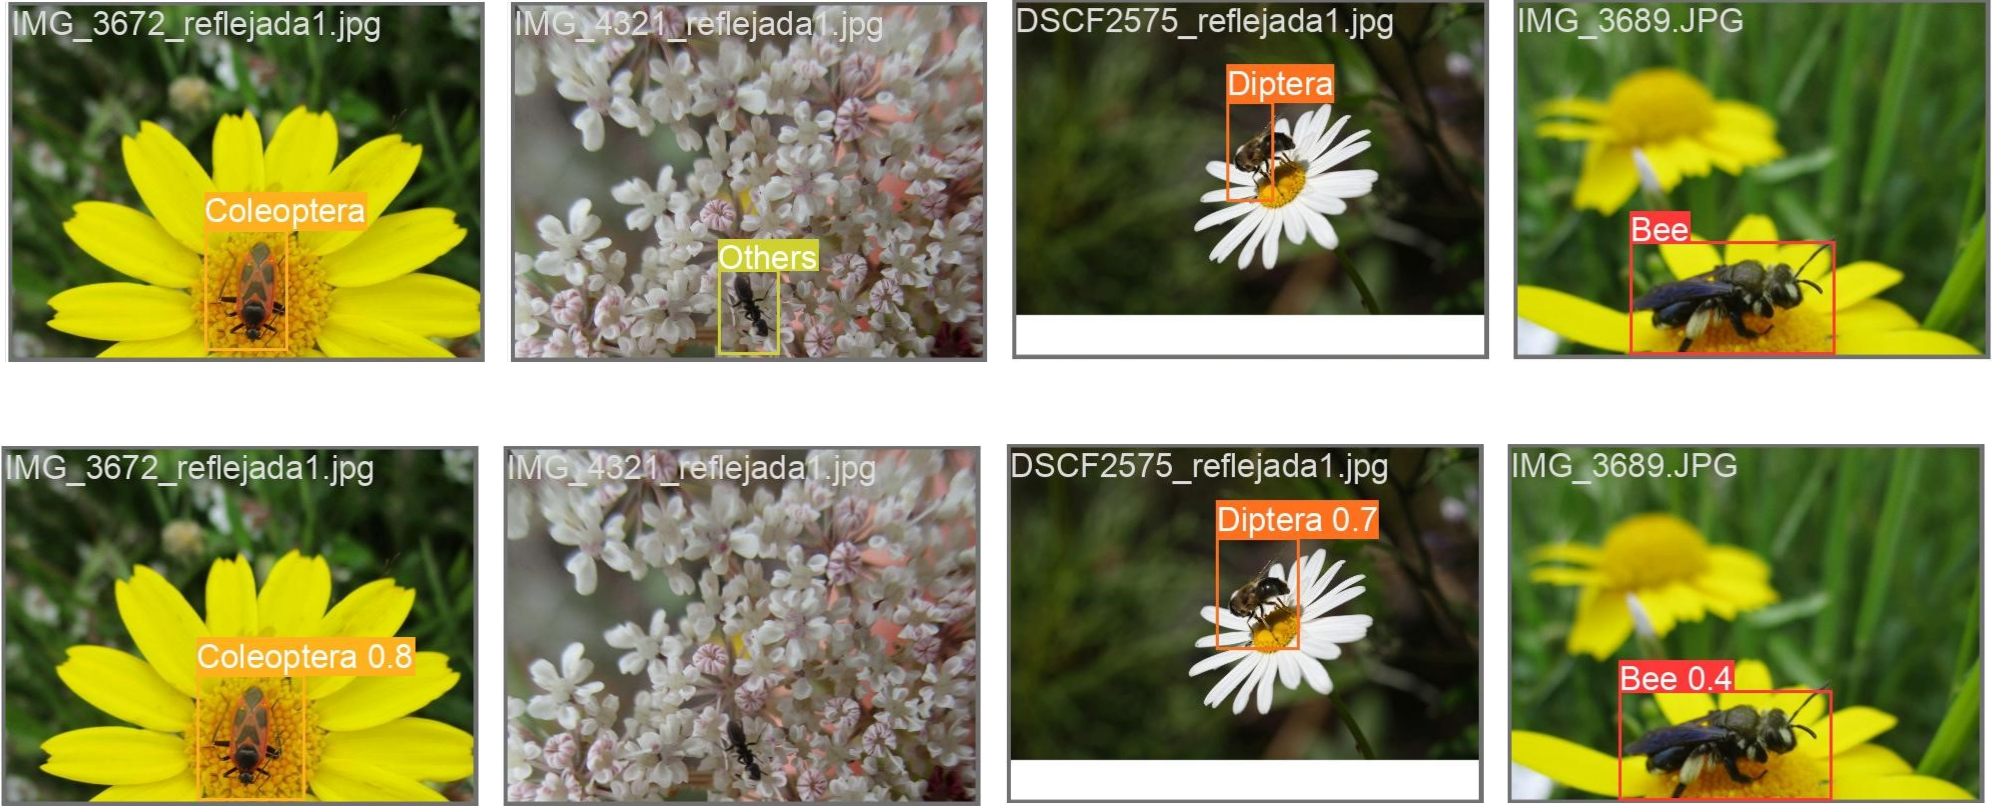
\includegraphics[width=0.98\textwidth]{Figuras/comparacion.png}
    \caption[Comparación entre detecciones realizadas por humanos y por el modelo YOLOv5.]{Comparación entre detecciones realizadas por humanos (arriba) y por el modelo YOLOv5 (abajo); el color muestra la categoría y el valor indica la confianza de la clasificación.}
    \label{fig:comparacion_humanos_yolov5}
\end{figure}


La Figura~\ref{fig:comparacion_humanos_yolov5} muestra una comparación entre la anotación manual (arriba) y las detecciones automatizadas realizadas por el modelo YOLOv5 (abajo). Es notable que en la categoría «Others», el modelo no logró detectar el insecto que sí fue identificado por un observador humano. En el caso de «Bee», el modelo proporciona un nivel de confianza relativamente bajo de 0.4, lo que podría indicar una menor certeza en su clasificación o una posible ambigüedad visual en la imagen. Sin embargo, en el caso de «Diptera», no solo la clasificación es correcta sino que la confianza es más alta (0.7), y el recuadro de detección parece más ajustado alrededor del insecto en comparación con la anotación humana. 

Finalmente, contando ya con el modelo entrenado, se procedió a realizar las detecciones en el conjunto de prueba. La matriz de confusión se puede apreciar en la Figura~\ref{fig:matriz_confusion_yolov5_prueba}. Se muestra una tendencia predominante hacia la no detección de insectos, más que hacia la confusión entre clases. Los valores significativos en la columna «Background» sugieren que el modelo frecuentemente clasifica regiones que contienen insectos como parte del fondo, particularmente en las categorías de «Coleoptera» y «Others». Sin embargo, en la confusión entre clases, se obtiene valores por debajo del 2 \%.

\begin{figure}[H]
    \centering
    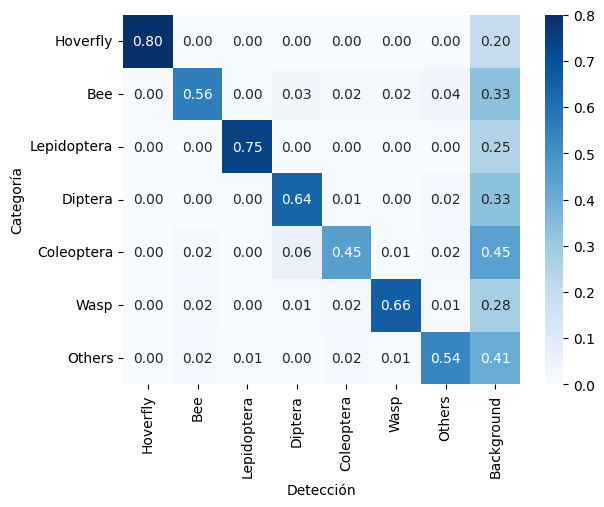
\includegraphics[width=0.75\textwidth]{Figuras/test_yolov5m_v01.png}
    \caption{Matriz de confusión del modelo YOLOv5 en el conjunto de prueba.}
    \label{fig:matriz_confusion_yolov5_prueba}
\end{figure}

Con esto, se calculó la precisión y exhaustividad por clase, los resultados pueden verse en la Tabla~\ref{tab:metricas}. La precisión se mantiene alta a través de todas las categorías, sobresaliendo en «Lepidoptera» con un 0.98, lo que refleja una fuerte capacidad del modelo para identificar correctamente las instancias positivas. No obstante, la exhaustividad presenta una variabilidad significativa; categorías como «Hoverfly» exhiben una alta concordancia entre precisión y exhaustividad (0.80), sugiriendo una detección equilibrada, mientras que otras como «Coleoptera» muestran una exhaustividad de solo 0.45, implicando una proporción considerable de falsos negativos.



\begin{table}[H]
    \centering\small
    \begin{tabular}{ccc}
        \toprule
        \textbf{Categoría} & \textbf{Precisión}  &  \textbf{Exhaustividad}\\ 
        \midrule
        Bee &  0.96 &  0.56 \\
        Coleoptera &  0.90 &  0.45 \\
        Diptera &  0.85 &  0.64 \\
        Hoverfly &  0.80 &  0.80 \\
        Lepidoptera &  0.98 &  0.75 \\
        Others &  0.79 &  0.54 \\
        Wasp &  0.82 &  0.66 \\
        \bottomrule
    \end{tabular}
    \caption{Métricas del modelo YOLOv5.}
    \label{tab:metricas}
\end{table}

\pagebreak

Adicionalmente, la exactitud global del modelo (\textit{accuracy}) es del 58 \%, lo cual refleja la proporción de predicciones correctas en relación con el total de predicciones realizadas. Este número es influido por todas las clases, por lo que la baja exhaustividad en algunas categorías puede afectar negativamente la exactitud general. 

Dado que la deficiencia del modelo se encuentra en la falta de detección de insectos en algunas imágenes, esto puede deberse a que los insectos son demasiado pequeños para ser detectados, por esta razón, se recalculó la precisión general del modelo, filtrando por el tamaño de los insectos. El cálculo de tamaño de los insectos se lo realizó tomando en cuenta el área de detección del insecto, medido en pixeles. Con esto, se obtuvieron los resultados que se presentan en la Tabla~\ref{tab:metricas_area}.

\begin{table}[H]
    \centering\small
    \begin{tabular}{ccc}
    \toprule
          \textbf{Área mínima (\%)} & \textbf{Cantidad de imágenes}  &  \textbf{Exactitud general}\\ 
    \midrule
        0.0 & 1891 & 0.58 \\
        0.1 & 1795 & 0.61 \\
        0.5 & 1489 & 0.66 \\
        1.0 & 1233 & 0.67 \\
        2.5 & 812 & 0.71 \\
        5.0 & 502 & 0.72 \\
        10.0 & 271 & 0.74 \\
    \bottomrule
    \end{tabular}
    \caption{Precisión general modelo YOLOv5 en función del área de detección.}
    \label{tab:metricas_area}
\end{table}

Con estos resultados se observa que, el tamaño del insecto incide de manera significativa en la precisión general de la clasificación. Un posible valor para tomar es que el insecto ocupe un espacio superior al 2.5 \% del área total de la imagen, en la cual se obtiene una exactitud general de 0.71. Con esto, se recalculó la matriz de confusión, la cual se puede apreciar en la Figura~\ref{fig:matriz_confusion_yolov5_prueba_area}. Adicionalmente, se recalculó la precisión y exhaustividad por clase, los resultados pueden verse en la Tabla~\ref{tab:metricas_area}. 


La nueva matriz de confusión (Figura~\ref{fig:matriz_confusion_yolov5_prueba_area}) tras el ajuste en el tamaño de los insectos detectados refleja una mejora notable en la detección de la categoría «Hoverfly», alcanzando una precisión del 100 \%. Adicionalmente, la todas las categorías, salvo «Others», muestran una mejora en los resultados, superando en todas el valor de 0.6. Aunque la no detección ha disminuido todas las categorías, persiste como un problema significativo, especialmente en «Others».

\begin{figure}[H]
    \centering
    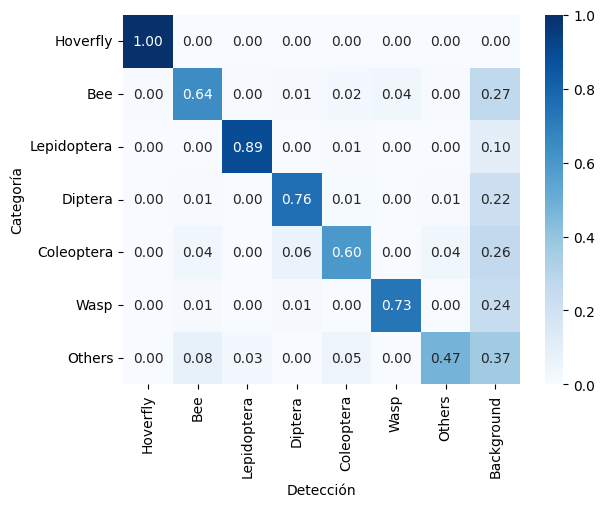
\includegraphics[width=0.75\textwidth]{Figuras/test_yolov5m_v01_area.png}
    \caption{Matriz de confusión del modelo YOLOv5 en el conjunto de prueba, con un área mínima del 2.5 \% del área total de la imagen.}
    \label{fig:matriz_confusion_yolov5_prueba_area}
\end{figure}


Por otro lado, el modelo muestra una mejora en la precisión para la mayoría de las categorías (ver Tabla~\ref{tab:metricas_area25}), con «Lepidoptera» alcanzando una precisión sobresaliente de 0.98 y una exhaustividad de 0.87.  Las categorías «Bee», «Coleoptera», y «Wasp» muestran una precisión alta, pero persiste un nivel de exhaustividad bajo, lo que indica que aún se pasan por alto instancias reales. La categoría «Others» continúa siendo la más desafiante para el modelo, con las métricas más bajas en precisión y exhaustividad, reflejando dificultades tanto en la detección como en la clasificación correcta.

\begin{table}[H]
    \centering\small
    \begin{tabular}{ccc}
    \toprule
          \textbf{Categoría} & \textbf{Precisión}  &  \textbf{Exhaustividad}\\ 
    \midrule
        Bee &  0.94 &  0.64 \\
        Coleoptera &  0.88 &  0.60 \\
        Diptera &  0.92 &  0.76 \\
        Hoverfly &  0.88 &  1.00 \\
        Lepidoptera &  0.98 &  0.87 \\
        Others &  0.72 &  0.47 \\
        Wasp &  0.86 &  0.73 \\
    \bottomrule
    \end{tabular}
    \caption{Métricas del modelo YOLOv5, con un área mínima del 2.5 \% del área total de la imagen.}
    \label{tab:metricas_area25}
\end{table}

\subsubsection{Validación cruzada}

Se implementó un enfoque de validación cruzada con 5 \textit{folds} para evaluar la generalización del modelo YOLOv5 en la tarea de clasificación. Este método consiste en dividir el conjunto de datos de forma aleatoria en cinco partes (o \textit{folds}), utilizando cuatro de ellas para el entrenamiento y la restante para la validación, repitiendo este proceso cinco veces de manera que cada \textit{folds} sirva una vez como conjunto de validación. 

Para integrar los resultados de los cinco modelos generados en la validación cruzada, se adoptó el criterio de unificarlos bajo la máxima media del nivel de confianza de las predicciones de cada modelo. Esto significa que, para cada observación, se seleccionó la predicción con la mayor confianza promedio entre los diferentes modelos. Este enfoque maximiza la certeza en las predicciones finales y contribuye a una evaluación más precisa de la estabilidad del modelo.

Con esto, se calculó la precisión y exhaustividad por clase, los resultados pueden verse en la Tabla~\ref{tab:metricas_cross}.

\begin{table}[H]
    \centering\small
    \begin{tabular}{ccc}
    \toprule
          \textbf{Categoría} & \textbf{Precisión}  &  \textbf{Exhaustividad}\\ 
    \midrule
        Bee &           0.89 &  0.69 \\
        Coleoptera &    0.91 &  0.55 \\
        Diptera &       0.85 &  0.70 \\
        Hoverfly &      0.32 &  0.70 \\
        Lepidoptera &   0.96 &  0.78 \\
        Others &        0.68 &  0.57 \\
        Wasp &          0.75 &  0.77 \\
    \bottomrule
    \end{tabular}
    \caption{Métricas del modelo YOLOv5, con validación cruzada.}
    \label{tab:metricas_cross}
\end{table}

Se presentan variaciones interesantes en comparación con los resultados originales. En la categoría «Bee», se observa una disminución en la precisión (de 0.96 a 0.89) pero un aumento en la exhaustividad (de 0.56 a 0.69), lo que indica una mejor identificación de esta categoría a costa de una precisión ligeramente reducida. Similarmente, en «Coleoptera» y «Diptera», la precisión se mantiene alta, con un notable aumento en la exhaustividad para «Diptera». Sin embargo, la categoría «Hoverfly», aunque muestra un aumento en la exhaustividad, tiene una precisión significativamente baja, posiblemente debido al número limitado de muestras. En contraste, la categoría «Others» muestra un descenso tanto en precisión como en exhaustividad.

La exactitud global del modelo mejoró notablemente, pasando de 0.58 en los resultados originales a 0.67 en la validación cruzada. Este incremento es un indicador positivo de que el modelo generaliza mejor sus predicciones a través de diferentes conjuntos de datos, lo que sugiere una robustez incrementada. Las fluctuaciones en precisión y exhaustividad, aunque son comunes en el proceso de validación y pruebas, indican que el modelo mantiene una buena capacidad de generalización. La mejora en la exactitud global, junto con los ajustes observados en otras métricas, sugiere que el modelo es confiable y efectivo, con un nivel de \textit{overfitting} controlado.

\subsection{EfficientNet}

Se siguió la misma metodología que en el modelo anterior. Se realizó una prueba con el modelo EfficientNetB7, con el fin de determinar si este era capaz de detectar los polinizadores en las imágenes. Para ello, se utilizó el conjunto de prueba para determinar las detecciones realizadas por el modelo; cabe recalcar que, el modelo EfficientNet \cite{tan-2019} está entrenado con el conjunto ImageNet, el cual no cuenta con polinizadores. Por esto, se obtuvieron diversos objetos detectados, los primeros diez objetos más detectados se pueden apreciar en la Tabla~\ref{tab:objetos_detectados_efficientnet}.

\begin{table}[H]
    \centering
    \begin{tabular}{cc}
        \toprule
        \textbf{Objeto} & \textbf{Cantidad} \\
        \midrule
        matchstick        &    779 \\
        jack-o'-lantern   &    233 \\
        nematode          &    181 \\
        daisy             &     80 \\
        abaya             &     66 \\
        spotlight         &     54 \\
        velvet            &     49 \\
        feather boa       &     31 \\
        candle            &     22 \\
        sea urchin        &     21 \\
        \bottomrule
    \end{tabular}
    \caption{Objetos detectados por el modelo EfficientNet.}
    \label{tab:objetos_detectados_efficientnet}
\end{table}

Con este resultado base, se procedió a entrenar el modelo EfficientNet con los datos de polinizadores. Para ello, se utilizó el conjunto de entrenamiento, y se validó con el conjunto de validación. El entrenamiento se realizó con 50 épocas, con un tamaño de lote de 32 imágenes, y con un tamaño de imagen de 600 píxeles, para esto, se realizó un reescalado de las imágenes. Adicionalmente, se agregó una capa \textit{softmax} al final del modelo, con el fin de realizar la clasificación de las detecciones.

Las curvas de aprendizaje obtenidas se pueden apreciar en la Figura~\ref{fig:curvas_aprendizaje_efficientnet}. Estas curvas muestran una precisión de entrenamiento y validación inusualmente bajas, lo que sugiere un posible subajuste y la necesidad de una optimización en el proceso de entrenamiento. La baja precisión, con valores fluctuantes entre 0.11 y 0.18, indica que el modelo tiene dificultades para captar las características distintivas de los datos.

\begin{figure}[H]
    \centering
    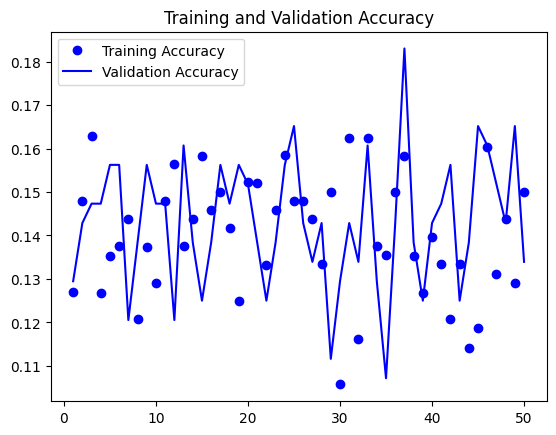
\includegraphics[width=0.49\textwidth]{Figuras/curvas_aprendizaje_efficientnet_1.png}
    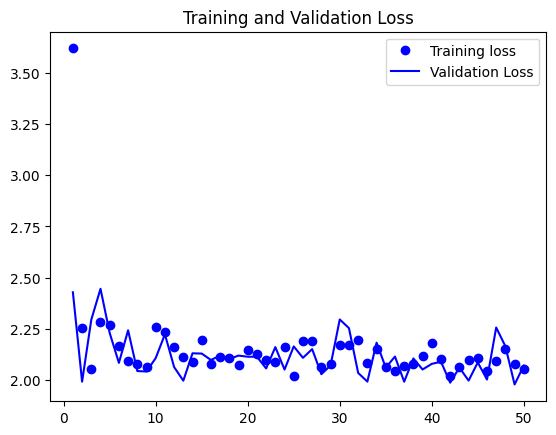
\includegraphics[width=0.49\textwidth]{Figuras/curvas_aprendizaje_efficientnet_2.png}
    \caption{Curvas de aprendizaje del modelo EfficientNet.}
    \label{fig:curvas_aprendizaje_efficientnet}
\end{figure}

Se puede apreciar que no existe un aprendizaje, esto puede deberse a que EfficientNet no toma en cuenta el bounding box de las imágenes, por lo que realiza una detección en general de la imagen, y no de los polinizadores en específico. Finalmente, contando ya con el modelo entrenado, se procedió a realizar las detecciones en el conjunto de prueba, sin resultados satisfactorios.

\section{Reconstrucción de red de polinizadores}

Con el modelo YOLOv5 entrenado, se procedió a realizar las detecciones en el conjunto de prueba. En este punto, solo se tomaron las imágenes originales, sin sus reflexiones. Se tiene un total de 1110 imágenes. Dentro de estas, el modelo detectó insectos en 701 imágenes. La distribución de los insectos en las imágenes se puede apreciar en la Figura~\ref{fig:distribucion_insectos}. Se observa que se tiene una distribución similar entre las observaciones reales y las estimaciones del modelo YOLOv5 para la mayoría de las categorías de insectos, lo que valida el buen funcionamiento del método aplicado. Sin embargo, es notable la discrepancia en la categoría «Bee», donde el modelo subestima claramente su presencia.

\begin{figure}[H]
    \centering
    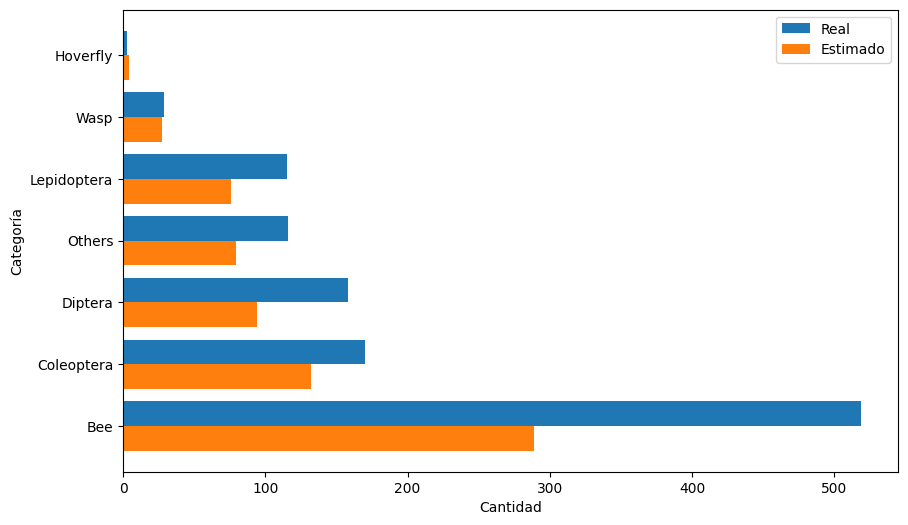
\includegraphics[width=0.835\textwidth]{Figuras/distribucion_insectos.png}
    \caption{Distribución de los insectos en las imágenes.}
    \label{fig:distribucion_insectos}
\end{figure}


Por el lado de las plantas, se utilizó la herramienta \textit{My PlantNet API} \cite{PlantNet} para la identificación de las plantas en las imágenes. A partir de los datos proporcionados por la API, se tomó la Familia de cada planta. En total, se detectaron 40 familias de plantas, la distribución de estas se puede apreciar en la Figura~\ref{fig:distribucion_familias}. Se puede apreciar que, la familia más abundante es \textit{Asteraceae}, con más de 300 imágenes. Por otro lado, existen algunas familias con una sola imagen.

\begin{figure}[H]
    \centering
    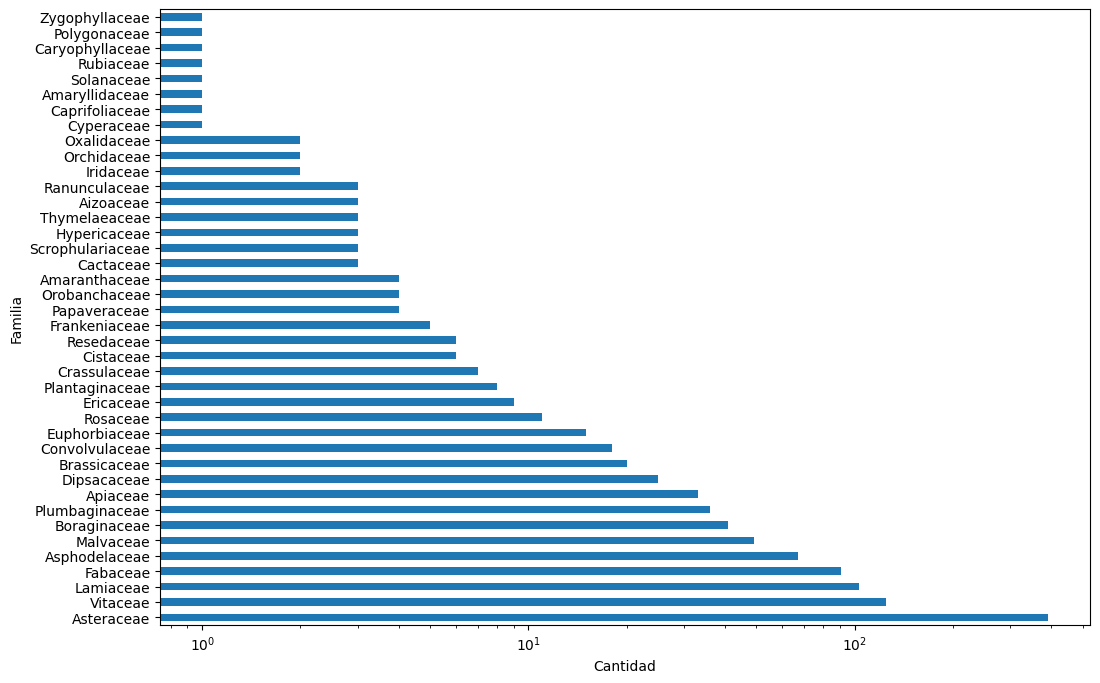
\includegraphics[width=0.885\textwidth]{Figuras/distribucion_familias.png}
    \caption{Distribución de las familias de plantas en las imágenes, en escala logarítmica.}
    \label{fig:distribucion_familias}
\end{figure}

Con esto, se llevó a cabo la construcción de dos redes planta-polinizador distintas. La primera red se derivó de las categorías identificadas a través de la observación humana, la cual se asume como el punto de referencia o red «real». Esta red proporciona una base para comparar la efectividad de las detecciones automáticas. La segunda red se generó a partir de las detecciones realizadas por el modelo YOLOv5. Al contrastar las dos redes, se puede evaluar no solo la capacidad de detección del modelo sino también su aplicabilidad en estudios ecológicos reales.

\subsection{Red planta-polinizador real}

La matriz de interacciones de la red real se puede apreciar en la Figura~\ref{fig:matriz_interacciones_real}. Se puede observar que, la mayoría de las especies interactúan con la especie «Bee», mientras que las especies «Hoverfly» y «Wasp» tienen pocas interacciones. 

\begin{figure}[H]
    \centering
    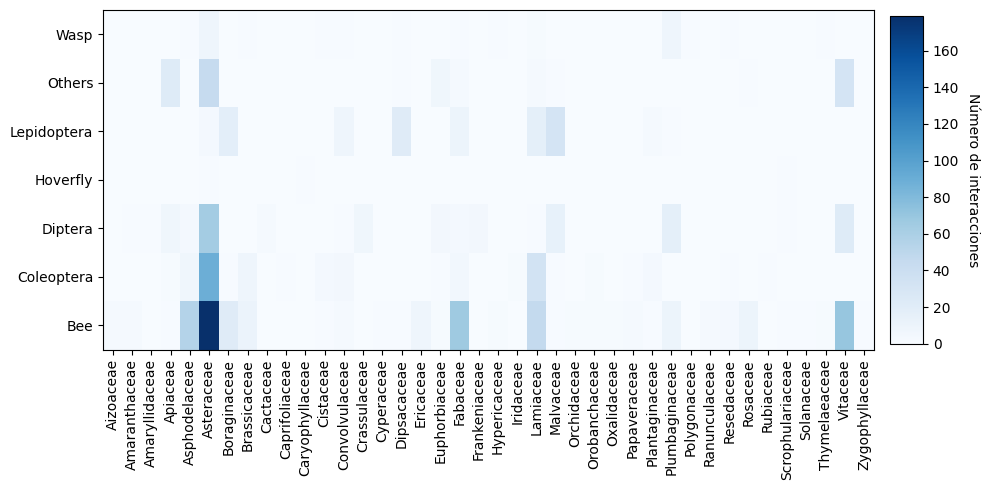
\includegraphics[width=0.96\textwidth]{Figuras/matriz_interacciones_real.png}
    \caption{Matriz de interacciones de la red real.}
    \label{fig:matriz_interacciones_real}
\end{figure}

A partir de esta matriz, con la metodología expuesta en el Capítulo~\ref{chapter:arte}, perteneciente a Young et al. \cite{young-2021}, se procedió a estimar la red real. El resultado de aplicar esta metodología es una matriz que contiene la probabilidad de conexión en el grafo, es decir, la probabilidad de que un insecto sea un polinizador de una planta. Esta matriz se puede apreciar en la Figura~\ref{fig:matriz_probabilidades_real}. 

\begin{figure}[H]
    \centering
    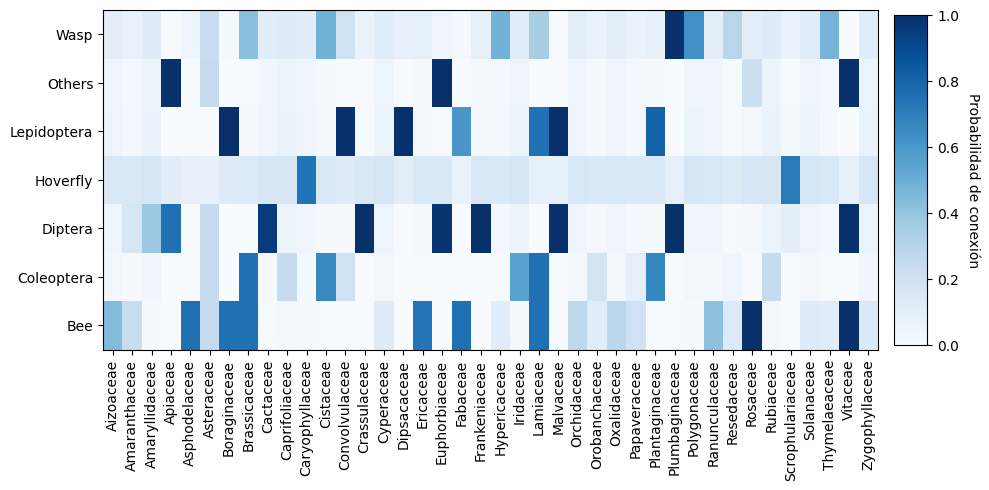
\includegraphics[width=0.96\textwidth]{Figuras/matriz_probabilidades_real.png}
    \caption{Matriz de probabilidades de la red real.}
    \label{fig:matriz_probabilidades_real}
\end{figure}

Seleccionando un umbral de confianza del 70 \%, se construyó la red planta-polinizador considerada como la red real. Este valor se eligió estratégicamente por ser el más alto que garantiza que cada especie de insecto conserva al menos una interacción con una planta, asegurando así la integridad biológica de la red. La visualización del resultado de esta estimación se presenta en la Figura~\ref{fig:red_real}. Con esto, se tiene que los insectos son polinizadores de únicamente 20 familias de plantas.

\begin{figure}[H]
    \centering
    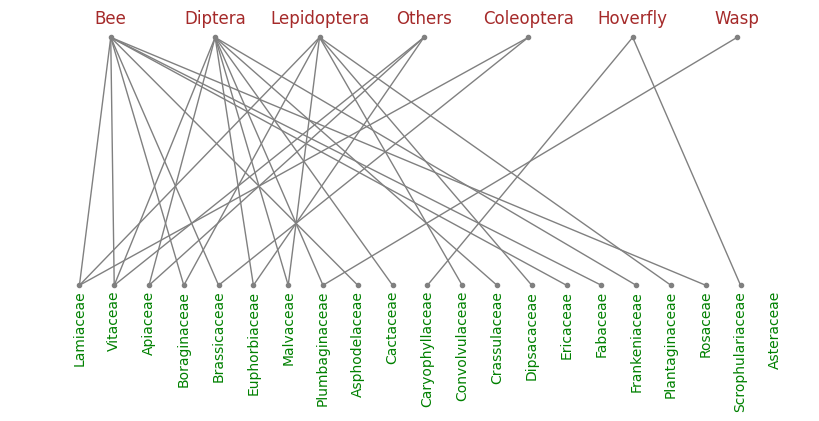
\includegraphics[width=0.95\textwidth]{Figuras/red_real.png}
    \caption{Red planta-polinizador real.}
    \label{fig:red_real}
\end{figure}


\subsection{Red planta-polinizador estimada}

La matriz de interacciones de la red estimada se puede apreciar en la Figura~\ref{fig:matriz_interacciones_estimada}. Se puede apreciar que tiene las mismas características que la matriz de interacciones de la red real, con la diferencia de que, en esta matriz, la clase «Coleoptera» posee menos interacciones que en la matriz de la red real.

\begin{figure}[H]
    \centering
    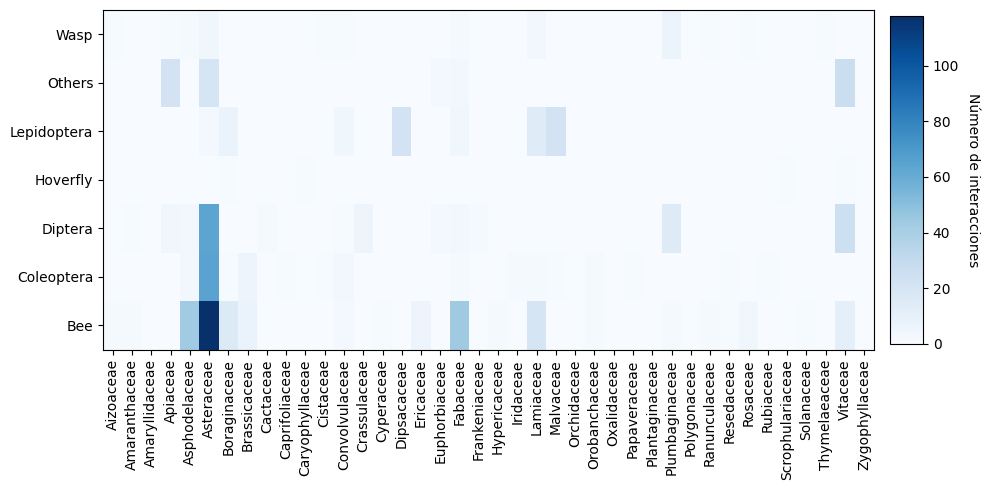
\includegraphics[width=0.96\textwidth]{Figuras/matriz_interacciones_estimada.png}
    \caption{Matriz de interacciones de la red estimada.}
    \label{fig:matriz_interacciones_estimada}
\end{figure}

A partir de esta matriz, al igual de lo descrito en la sección anterior, se procedió a estimar la red estimada. Con esto, se obtuvo la matriz de probabilidades de la red estimada, la cual se puede apreciar en la Figura~\ref{fig:matriz_probabilidades_estimada}.

\begin{figure}[H]
    \centering
    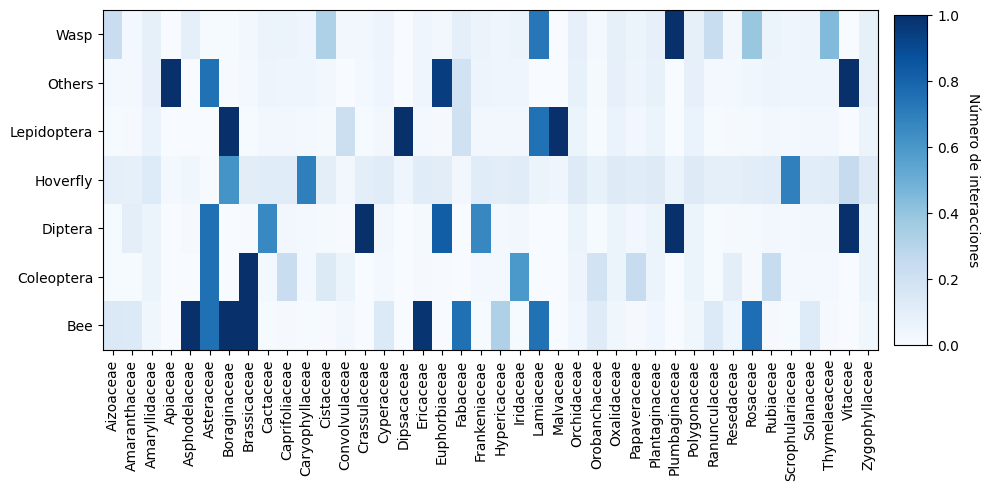
\includegraphics[width=0.96\textwidth]{Figuras/matriz_probabilidades_estimada.png}
    \caption{Matriz de probabilidades de la red estimada.}
    \label{fig:matriz_probabilidades_estimada}
\end{figure}

Tomando un nivel de confianza del 70 \%, se procedió a generar la red estimada. El resultado de esta estimación se puede apreciar en la Figura~\ref{fig:red_estimada}.

\begin{figure}[H]
    \centering
    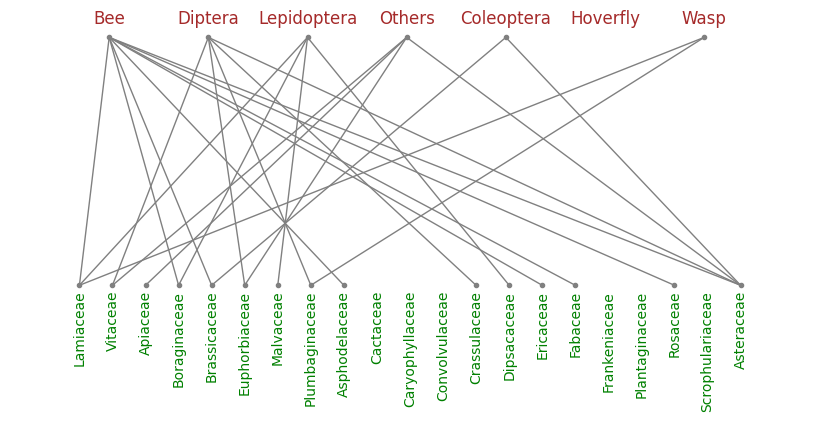
\includegraphics[width=0.95\textwidth]{Figuras/red_estimada.png}
    \caption{Red estimada.}
    \label{fig:red_estimada}
\end{figure}



\section{Comparación de redes}

Para la comparación de las redes, se tomará la componente conexa máximas de cada red. Para una comparación visual, se presentan la gráfica de ambas redes en la Figura~\ref{fig:redes_comparacion}. 

\begin{figure}[H]
    \centering
    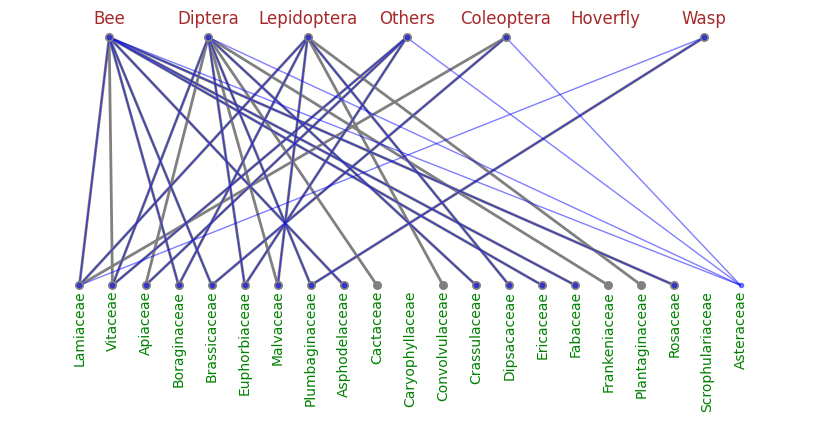
\includegraphics[width=0.95\textwidth]{Figuras/redes_comparacion.png}
    \caption[Comparación de las redes real y estimada.]{Comparación de las redes, en gris la red real y en azul la red estimada.}
    \label{fig:redes_comparacion}
\end{figure}

Se puede apreciar que, la red estimada posee una mayor cantidad de nodos y aristas que la red real. Por otro lado, se observa que, en la red estimada, la familia \textit{Asteraceae} tiene una presencia mayor que en la red real.

Para comenzar el análisis cuantitativo de las redes planta-polinizador, se examinan los datos básicos de la red real y la red estimada. En la Tabla~\ref{tab:metricas_redes} se presentan las métricas de ambas redes. La red real cuenta con 24 nodos y 28 aristas, lo que sugiere una estructura de red con una variedad de especies y conexiones. Por otro lado, la red estimada presenta una ligera reducción con 21 nodos y 25 aristas, lo que podría indicar que el modelo de estimación no capturó todas las interacciones o especies presentes en la red real.

\begin{table}[H]
    \centering\small
    \begin{tabular}{ccc}
    \toprule
          \textbf{Métrica} & \textbf{Red real}  &  \textbf{Red estimada}\\ 
    \midrule
        Nodos &  24 &  21 \\
        Aristas &  28 &  25 \\
        Densidad &  0.101 &  0.119 \\
        Grado medio & 2.33 & 2.38 \\
    \bottomrule
    \end{tabular}
    \caption{Métricas de las redes.}
    \label{tab:metricas_redes}
\end{table}

La densidad de la red, que proporciona una idea de cuán conectada está la red, es ligeramente mayor en la red estimada (0.119) en comparación con la red real (0.101). Esto implica que, proporcionalmente, la red estimada tiene una mayor propensión de conexiones entre sus nodos respecto al número total de conexiones posibles. El grado medio, que es el número promedio de conexiones por nodo, es similar en ambas redes, con 2.33 para la red real y 2.38 para la red estimada, lo que indica que, en promedio, cada especie en ambas redes tiende a interactuar con un número comparable de otras especies.

Para analizar la similitud entre los grafos de las redes real y estimada, se procedió a calcular el distancias de \textit{error de desplazamiento} (MDE) y la \textit{similitud del coseno}, entre las filas de las matrices de adyacencia de los grafos. Estas dos métricas que ofrecen perspectivas distintas sobre la comparación de las matrices de adyacencia de los grafos. El error de desplazamiento mide la diferencia promedio en las conexiones entre dos grafos; un valor bajo indica que las posiciones de las conexiones en un grafo son muy similares a las del otro. Se calcula tomando la diferencia absoluta entre las matrices de adyacencia de los dos grafos, elemento por elemento, y luego obteniendo la media de estas diferencias. Por otro lado, la similitud del coseno mide el coseno del ángulo entre dos vectores en un espacio multidimensional que, en este caso, son las filas de las matrices de adyacencia de los grafos. Esta métrica varía de -1 a 1, donde 1 indica que los dos vectores son idénticos en orientación, y un valor cercano a 1 sugiere una alta similitud entre los patrones de conexión de los grafos. Los resultados de estas distancias se pueden apreciar en la Tabla~\ref{tab:metricas_redes_2}.

\begin{table}[H]
    \centering\small
    \begin{tabular}{cc}
    \toprule
          \textbf{Distancia} & \textbf{Valor}  \\
    \midrule
        Error de desplazamiento &  0.053 \\
        Similitud del coseno &  0.972 \\
    \bottomrule
    \end{tabular}
    \caption{Distancia entre las redes.}
    \label{tab:metricas_redes_2}
\end{table}


Los resultados obtenidos de estas medidas indican una alta similitud entre los grafos de las redes real y estimada. Un error de desplazamiento medio de aproximadamente 0.053 sugiere que las diferencias promedio en las conexiones entre los dos grafos son mínimas, lo que implica que la ubicación de las conexiones en la red estimada corresponde estrechamente a la red real. Además, una similitud del coseno media de aproximadamente 0.972 confirma esta observación, indicando que la orientación de los vectores (o las filas de las matrices de adyacencia) es muy similar. 






\chapter{Conclusiones y trabajo futuro}
\label{chapter:conclusiones}

Este trabajo ha demostrado con éxito el desarrollo y la aplicación de una red neuronal convolucional (YOLOv5) para el reconocimiento automático de polinizadores en imágenes de flores, un paso significativo en la reconstrucción de redes planta-polinizador. Se ha procesado y analizado un conjunto de datos compuesto por 5445 imágenes, con especial atención en la estandarización del tamaño de las imágenes y la extracción precisa de información relevante mediante archivos XML.

Los resultados obtenidos del modelo YOLOv5 destacan una notable capacidad para detectar y clasificar polinizadores, aunque con ciertas limitaciones en la detección precisa de algunas especies y la diferenciación entre insectos y su entorno. Sin embargo, el uso de un tamaño mínimo de detección ha mejorado significativamente la precisión del modelo.

En lo que respecta a la validación cruzada para el modelo YOLOv5, los resultados obtenidos son alentadores y reflejan la robustez y la capacidad de generalización del modelo. A pesar de ciertas variaciones en la precisión y la exhaustividad entre las categorías, estas fluctuaciones son normales y esperadas en el proceso de validación.

Por otro lado, el modelo EfficientNet no logró un rendimiento satisfactorio, sugiriendo la necesidad de un enfoque más especializado para este tipo de datos.

En cuanto a la reconstrucción de redes de polinizadores, el análisis comparativo entre la red real y la estimada por el modelo ha proporcionado una visión valiosa sobre la eficacia de estas técnicas en la representación precisa de las interacciones en ecosistemas.

Las métricas calculadas sobre las redes muestran que el modelo ha hecho un trabajo notable al reproducir la estructura de la red planta-polinizador y que las diferencias entre las redes real y estimada son, en promedio, insignificantes. Esto sugiere que el modelo puede ser una herramienta confiable para la estimación de redes ecológicas.


Para trabajos futuros, se recomienda:

\begin{itemize}
\item 
    Exploración de Nuevas Técnicas y Modelos: Investigar otras arquitecturas de redes neuronales y métodos de procesamiento de imágenes que puedan mejorar la precisión en la detección y clasificación de polinizadores, especialmente en casos difíciles.
\item 
    Optimización de Modelos Existentes: Mejorar el entrenamiento y ajuste de modelos como EfficientNet para aumentar su eficacia en la detección de polinizadores.
\item 
    Ampliación de la Base de Datos: Incluir más variedades de polinizadores y plantas para enriquecer el conjunto de datos y permitir una generalización más robusta de los modelos.
\item 
    Aplicaciones en Conservación de la Biodiversidad: Explorar cómo estos modelos pueden aplicarse en proyectos de conservación y estudios de biodiversidad para comprender mejor las interacciones planta-polinizador.
\item 
    Generar protocolos para generar la detección de imágenes y la construcción de redes planta-polinizador a partir del trabajo de campo.
\end{itemize}

\appendix
\chapter{Anexos}
\label{chapter:Anexos}

\section{Repositorio GitHub}
\label{anexo:github}

En el siguiente enlace, se puede acceder al repositorio de GitHub donde se puede encontrar los notebooks con el código necesario para replicar los resultados presentados en este proyecto.
\begin{quote}
    \url{https://github.com/andres-merino/TFM-UOC-CienciaDeDatos}
\end{quote}
De manera específica, los \textit{notebooks} que se pueden encontrar son los siguientes:

\begin{itemize}
    \item \texttt{EfficientNET.ipynb}: \textit{notebook} con el código necesario para realizar el entrenamiento del modelo EfficientNet.
    \item \texttt{YOLOv5-entrenamiento.ipynb}: \textit{notebook} con el código necesario para realizar el entrenamiento del modelo YOLOv5, este fue ejecutado en Google Colab.
    \item \texttt{YOLOv5-prediccion.ipynb}: \textit{notebook} con el código necesario para realizar la predicción del modelo YOLOv5.
    \item \texttt{YOLOv5-prediccion-CrossVal.ipynb}: \textit{notebook} con el código necesario para realizar la predicción del modelo YOLOv5 con validación cruzada.
    \item \texttt{EstimacionRedPolinizadores.ipynb}: \textit{notebook} con el código necesario para realizar la estimación de la red de polinizadores.
    \item \texttt{RedPolinizadores.ipynb.ipynb}: \textit{notebook} con el código necesario para realizar el análisis de la red de polinizadores.
\end{itemize}


\section{Repositorio de pesos de modelos}
\label{anexo:pesos}

En el siguiente enlace, se puede acceder al repositorio particular de OneDrive del autor donde se puede encontrar los pesos de los modelos entrenados en este proyecto.
\begin{quote}
    \url{https://1drv.ms/f/s!AuK-ajP1UCYfoPF4K2pFOxNCGibnJg?e=RXUcK4}
\end{quote}
De manera específica, los pesos que se pueden encontrar son los siguientes:

\begin{itemize}
    \item \texttt{efficientnetb7\_weights.h5}: pesos del modelo EfficientNet.
    \item \texttt{yolov5m\_v01.pt}: pesos del modelo YOLOv5, en su versión \texttt{m}.
    \item \texttt{yolov5l\_v01.pt}: pesos del modelo YOLOv5 en su versión \texttt{l}.
    \item \texttt{yolov5m\_foldn.pt}: pesos del modelo YOLOv5 en el \textit{fold} \texttt{n} de la validación cruzada.
\end{itemize}




% bibliografia
% \nocite{*}
\addcontentsline{toc}{chapter}{Bibliografía}
% \bibliographystyle{plain}
\bibliographystyle{unsrt}
\bibliography{referencias.bib}

\end{document}
